\RequirePackage[final]{graphicx} 

\title{Modeling Autonomic Pupillary Responses from External Stimuli Using Machine Learning}

% \author{
% Shawhin Talebi $^{\dagger,*}$, David J. Lary $^{\dagger}$,ֿֿֿ\\
% Lakitha O. H. Wijerante $^{\dagger}$, and Tatiana Lary$^{\dagger}$
% }

\author{
Shawhin Talebi, David J. Lary,ֿֿֿ\\
Lakitha O. H. Wijerante, and Tatiana Lary
}

\documentclass[10pt]{article}

\usepackage{amssymb}
\usepackage[utf8]{inputenc}
\usepackage[english]{babel}
\usepackage[numbers,sort&compress]{natbib}
\usepackage{hyperref}

\begin{document}
\maketitle

\begin{abstract}
The human body exhibits a variety of autonomic responses. For example, changing light intensity provokes a change in the pupil dilation \cite{PupilLight}. In the past, formulae for pupil size based on luminance have been derived using traditional empirical approaches \cite{PupilModels}. In this paper, we present a different approach to a similar task by using machine learning to examine the multivariate non-linear autonomic response of pupil dilation as a function of a comprehensive suite of more than four hundred environmental parameters leading to the provision of quantitative empirical models. The objectively optimized empirical machine learning models use a multivariate non-linear non-parametric supervised regression algorithm employing an ensemble of regression trees which receive input data from both spectral and biometric data. The models for predicting the participant's pupil diameters from the input data had a fidelity of at least 96.9\% for both the training and independent validation data sets. The most important inputs were the light levels (illuminance) of the wavelengths near 562 nm. This coincides with the peak sensitivity of the long-wave photosensitive cones in the retina, which exhibit a maximum absorbance around \hbox{$\lambda_{max}$ = 562.8 $\pm$ 4.7 nm} \cite{BowmakerCones}. Both data and code are provided for easy replication of our results.
\end{abstract}


% Keywords
%\keyword{Machine Learning 1; Biometrics 2; Light Spectra 3; Pupillary Response 4}

\section{Introduction}

% This study is the first of a broader investigation
This study is part of a broader investigation into the role of the environment in influencing human physical and cognitive performance. The main purpose of this paper is to provide a baseline which accurately describes how changing illuminance affects pupil dilation, so that when  emotional or cognitive factors are also involved, we can start to discern the relative roles of illuminance  and cognitive load in affecting the pupil dilation. The ranking of the importance of the predictor variables used in our empirical machine learning models provides a useful metric of which variables are the key drivers,  providing us with valuable insights. 

The autonomic nervous system (ANT) is responsible for changes in pupil dilation. The changes in pupil dilation may occur due to changing light intensity, cognitive load and emotional load \cite{PupilReview}. While the light intensity allows an immediate response at the retinal level, an emotional and especially cognitive response, require some higher level processing. So, when the visual input is sent from the eye to the visual cortex via the optic nerve, it first goes through the thalamus. If at this point an imminent threat is detected, it responds mobilizing the body for a \lq fight or flight' response, which is then reflected in the changes in the pupil size. As the visual information is relayed to the visual center of the brain in the occipital lobe, it is further sent for processing via various routes to different parts of the brain. In a fast paced changing environment, executive function in the prefrontal lobes make decisions in a fraction of a second. This process also effects changes in pupil dilation. Some areas of the brain involved in the processing of cognitive and emotional load are deep seated structures and can only be observed by expensive equipment such as fMRI in an artificial lab setting. So part of the question we are starting to address in this study is \textit{how can we tell the difference to which stimuli the pupil is responding?} This study begins to answer this question using non-invasive methods that can be used in a natural setting by providing a methodology to accurately model the change in pupil size as a function of key environmental variables, so that when other changes are also occurring simultaneously (such as emotional and cognitive load) we can start to examine how these factors modify the pupil dilation response that occurs.

\begin{figure}[!t]
    \centering
    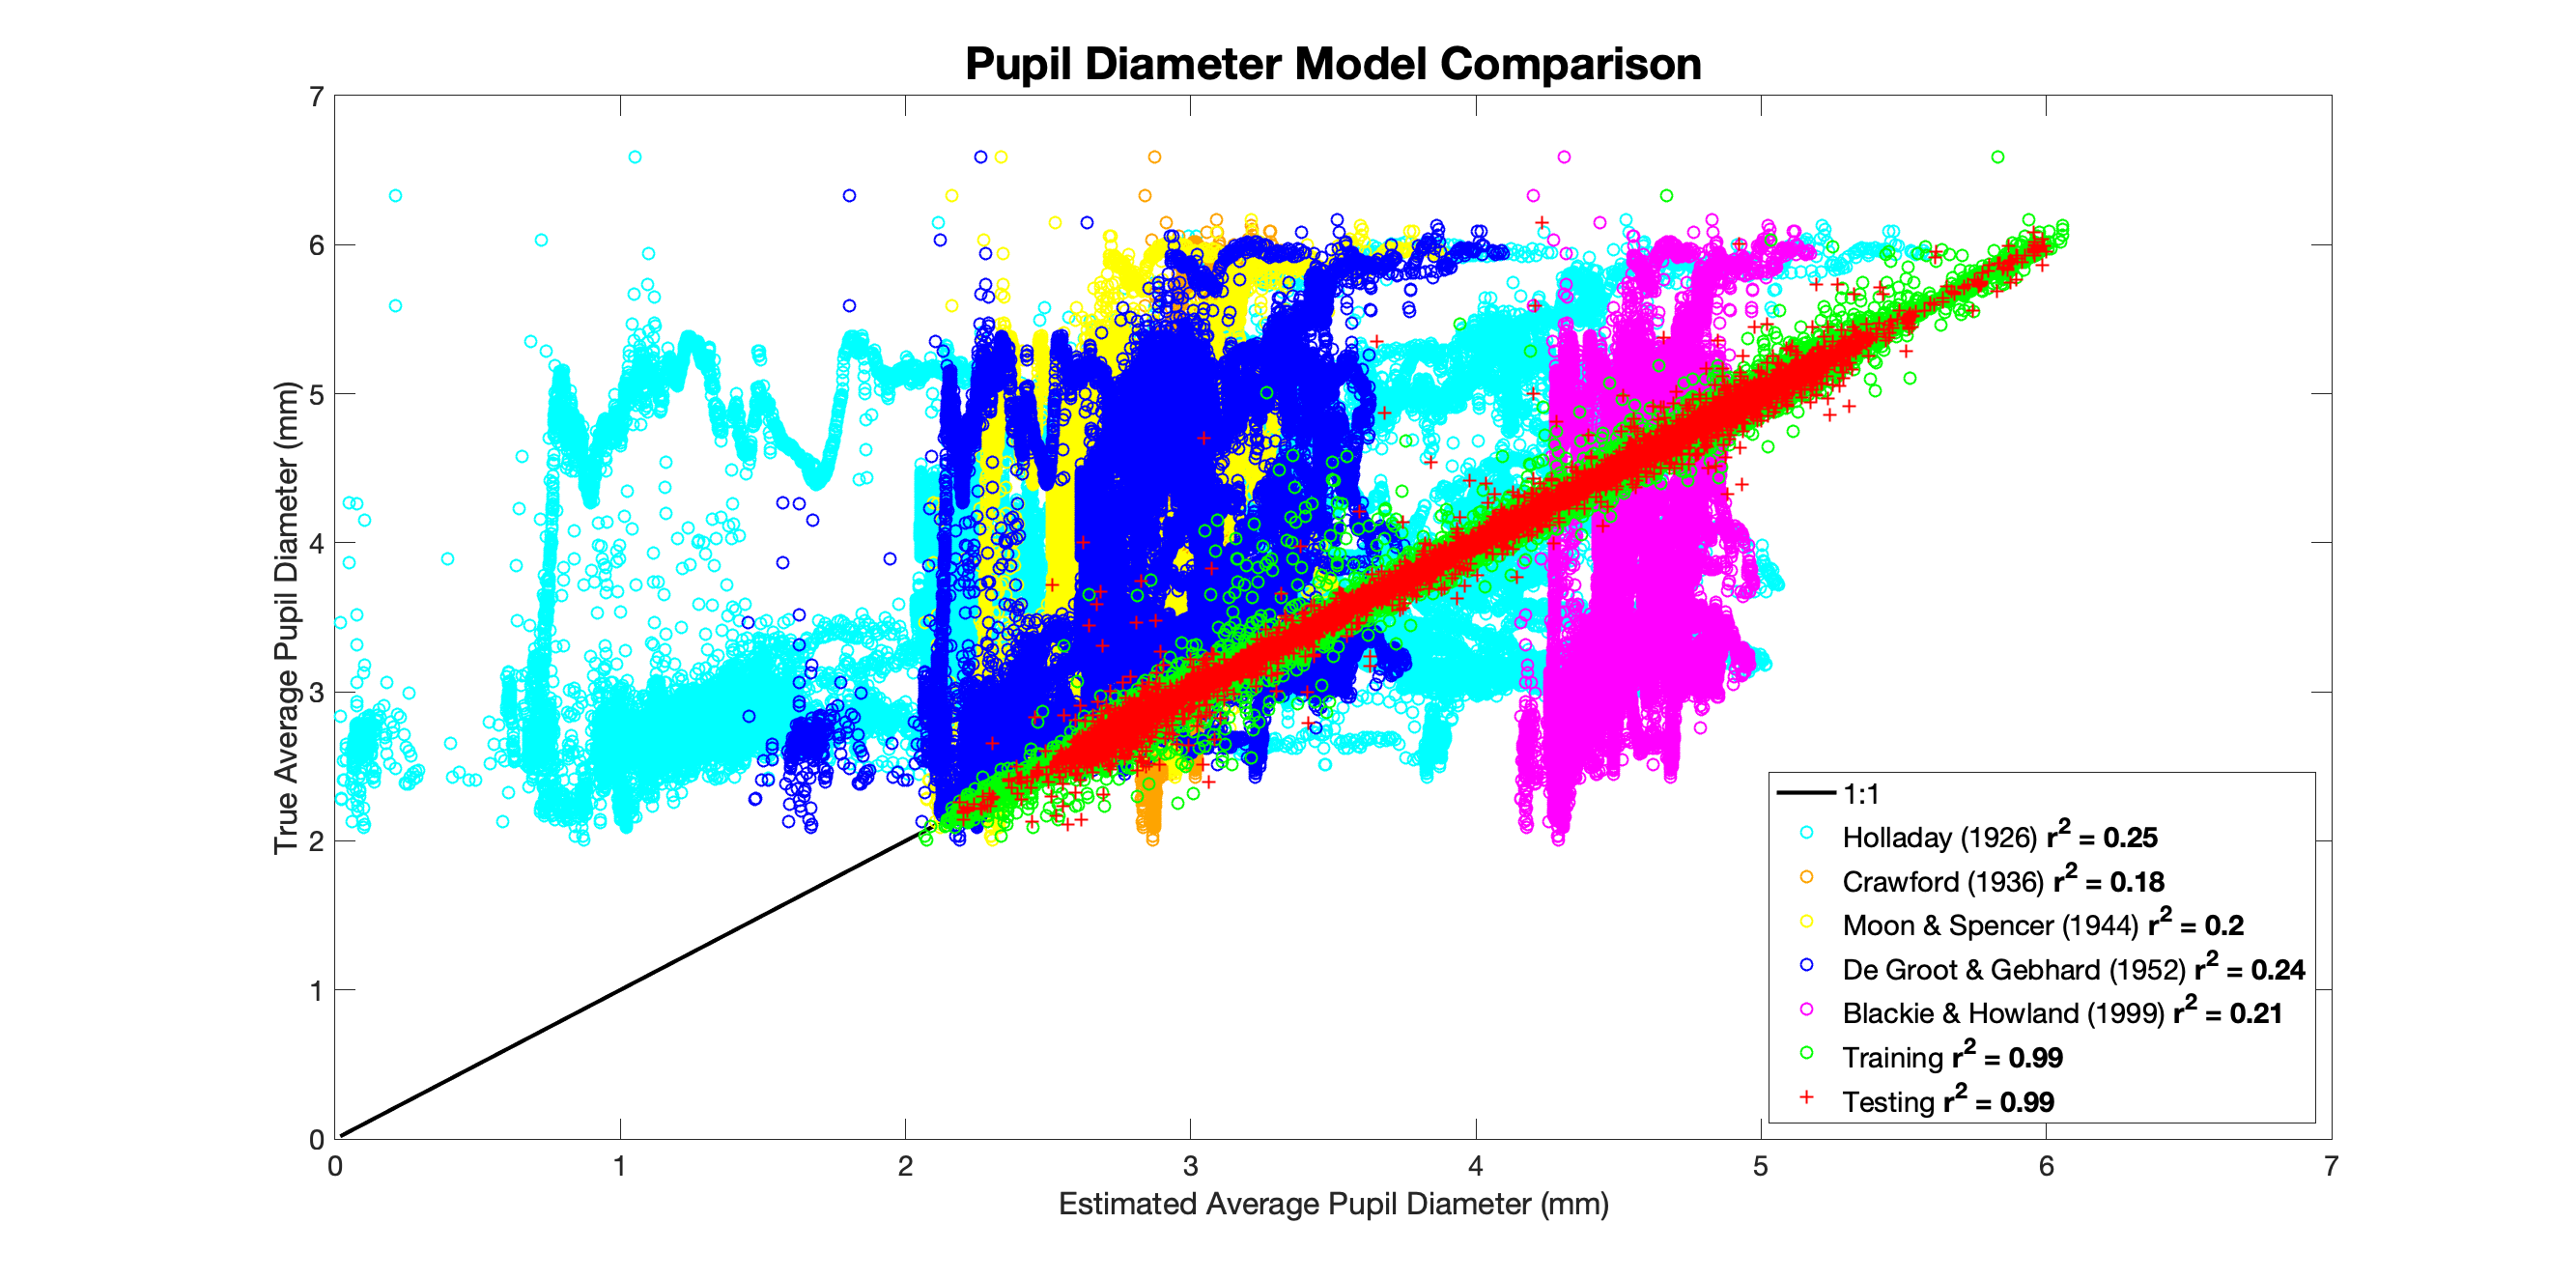
\includegraphics[width=0.95\textwidth]{./scatterPlots/OldModelsPlot.png}
    \caption{Evaluation and comparison of previous pupil diameter models which utilized a single variable, luminance, showing poor fidelity contrasted with the multivariate empirical machine learning model for the average pupil diameter developed in this study showing good fidelity (foreground green training and red validation points). The true average diameter of the left and right pupils is given on the y-axis, and the estimation by each respective model on the x-axis. Luminance was computed from measured illuminance where the luminance was assumed to be isotropic and reflectance assumed to be 1. Models were evaluated based on description by Watson and Yellott \cite{PupilModels}.}
    \label{fig:oldModels}
\end{figure}

 In addition to changes in pupil dilation, other autonomic responses include changes in heart rate variability, galvanic skin response (or sweating), and core temperature  \cite{HRVreview, GSR, tempLoad}. Each of these responses are influenced by variables such as cognitive load \cite{PupilLoad1,PupilLoad2,PupilLoad3,PupilLoad4}, age \cite{PupilAge}, pain level \cite{PupilPain}, and emotional state \cite{PupilEmotion}. In several previous studies formulae for pupil size utilized a single variable, luminance \cite{HolladayPupil1vModel, CrawfordPupil1vModel, MoonPupil1vModel, deGrootPupil1vModel, BlackiePupil1vModel}. A major shortcoming of these models is their lack of generality. This is illustrated in Figure \ref{fig:oldModels}, where the true pupil diameter is plotted against the estimated pupil diameter provided by each of the models enumerated in the legend. There is a clear contrast between the diffuse \textit{cloud} of data points from previous model predictions and the high fidelity predictions of the machine learning model developed here, shown by the green (training points) and the red (independent validation points) in the foreground. Of the five previous models, Holladay's formula \cite{HolladayPupil1vModel} performed the best, with a fidelity of $\approx$ 25\%. The substantial error of these previous models is a likely reflection of both missing parameters being missing and the challenge of finding the exact functional form required for predicting the pupil diameter. Later models added variables such as adaptation field, age, and monocular adaptation \cite{StanleyPupilMvModel,BartenPupilMvModel,PupilModels}. All of the earlier models considered ambient light levels by way of the total luminance as opposed to the fine wavelength resolution of the UV/visible spectrum that was used in this study. The fine wavelength resolution allows one to identify the wavelengths to which the pupil dilation is most sensitive, it is noteworthy that there are some small variations from eye to eye in the key wavelengths for determining the pupil diameter. In this study we have utilized recent technological developments, the full visible spectrum and pupil size can be measured with high accuracy and in large volume combined with machine learning, this provides new opportunities for the development of much more robust higher fidelity empirical models.

In this first demonstration case study, with just one participant, we examined the effect of both light intensity and the orientation/motion of the head on the diameter of a participant's pupils. Different illumination environments can be characterized by their spectra. This light consisting of various wavelengths which can interact with different photo-receptors (light sensitive cones) in the retina. This interaction produces electrical signals that are sent to the brain and interpreted as color \cite{LightColor}. These cones are disproportionately sensitive to particular wavelengths with absorbance peaks around 420 nm (violet), 534 nm (green), and 564 nm (yellow-green) \cite{BowmakerCones}. An illustration of these sensitivities can be shown by a plot of the mean absorbance of the three classes of photo-receptors (short-wave, middle-wave, and long-wave cones) vs wavelength (shown in Figure \ref{fig:absorbances}).

\begin{figure}[!t]
    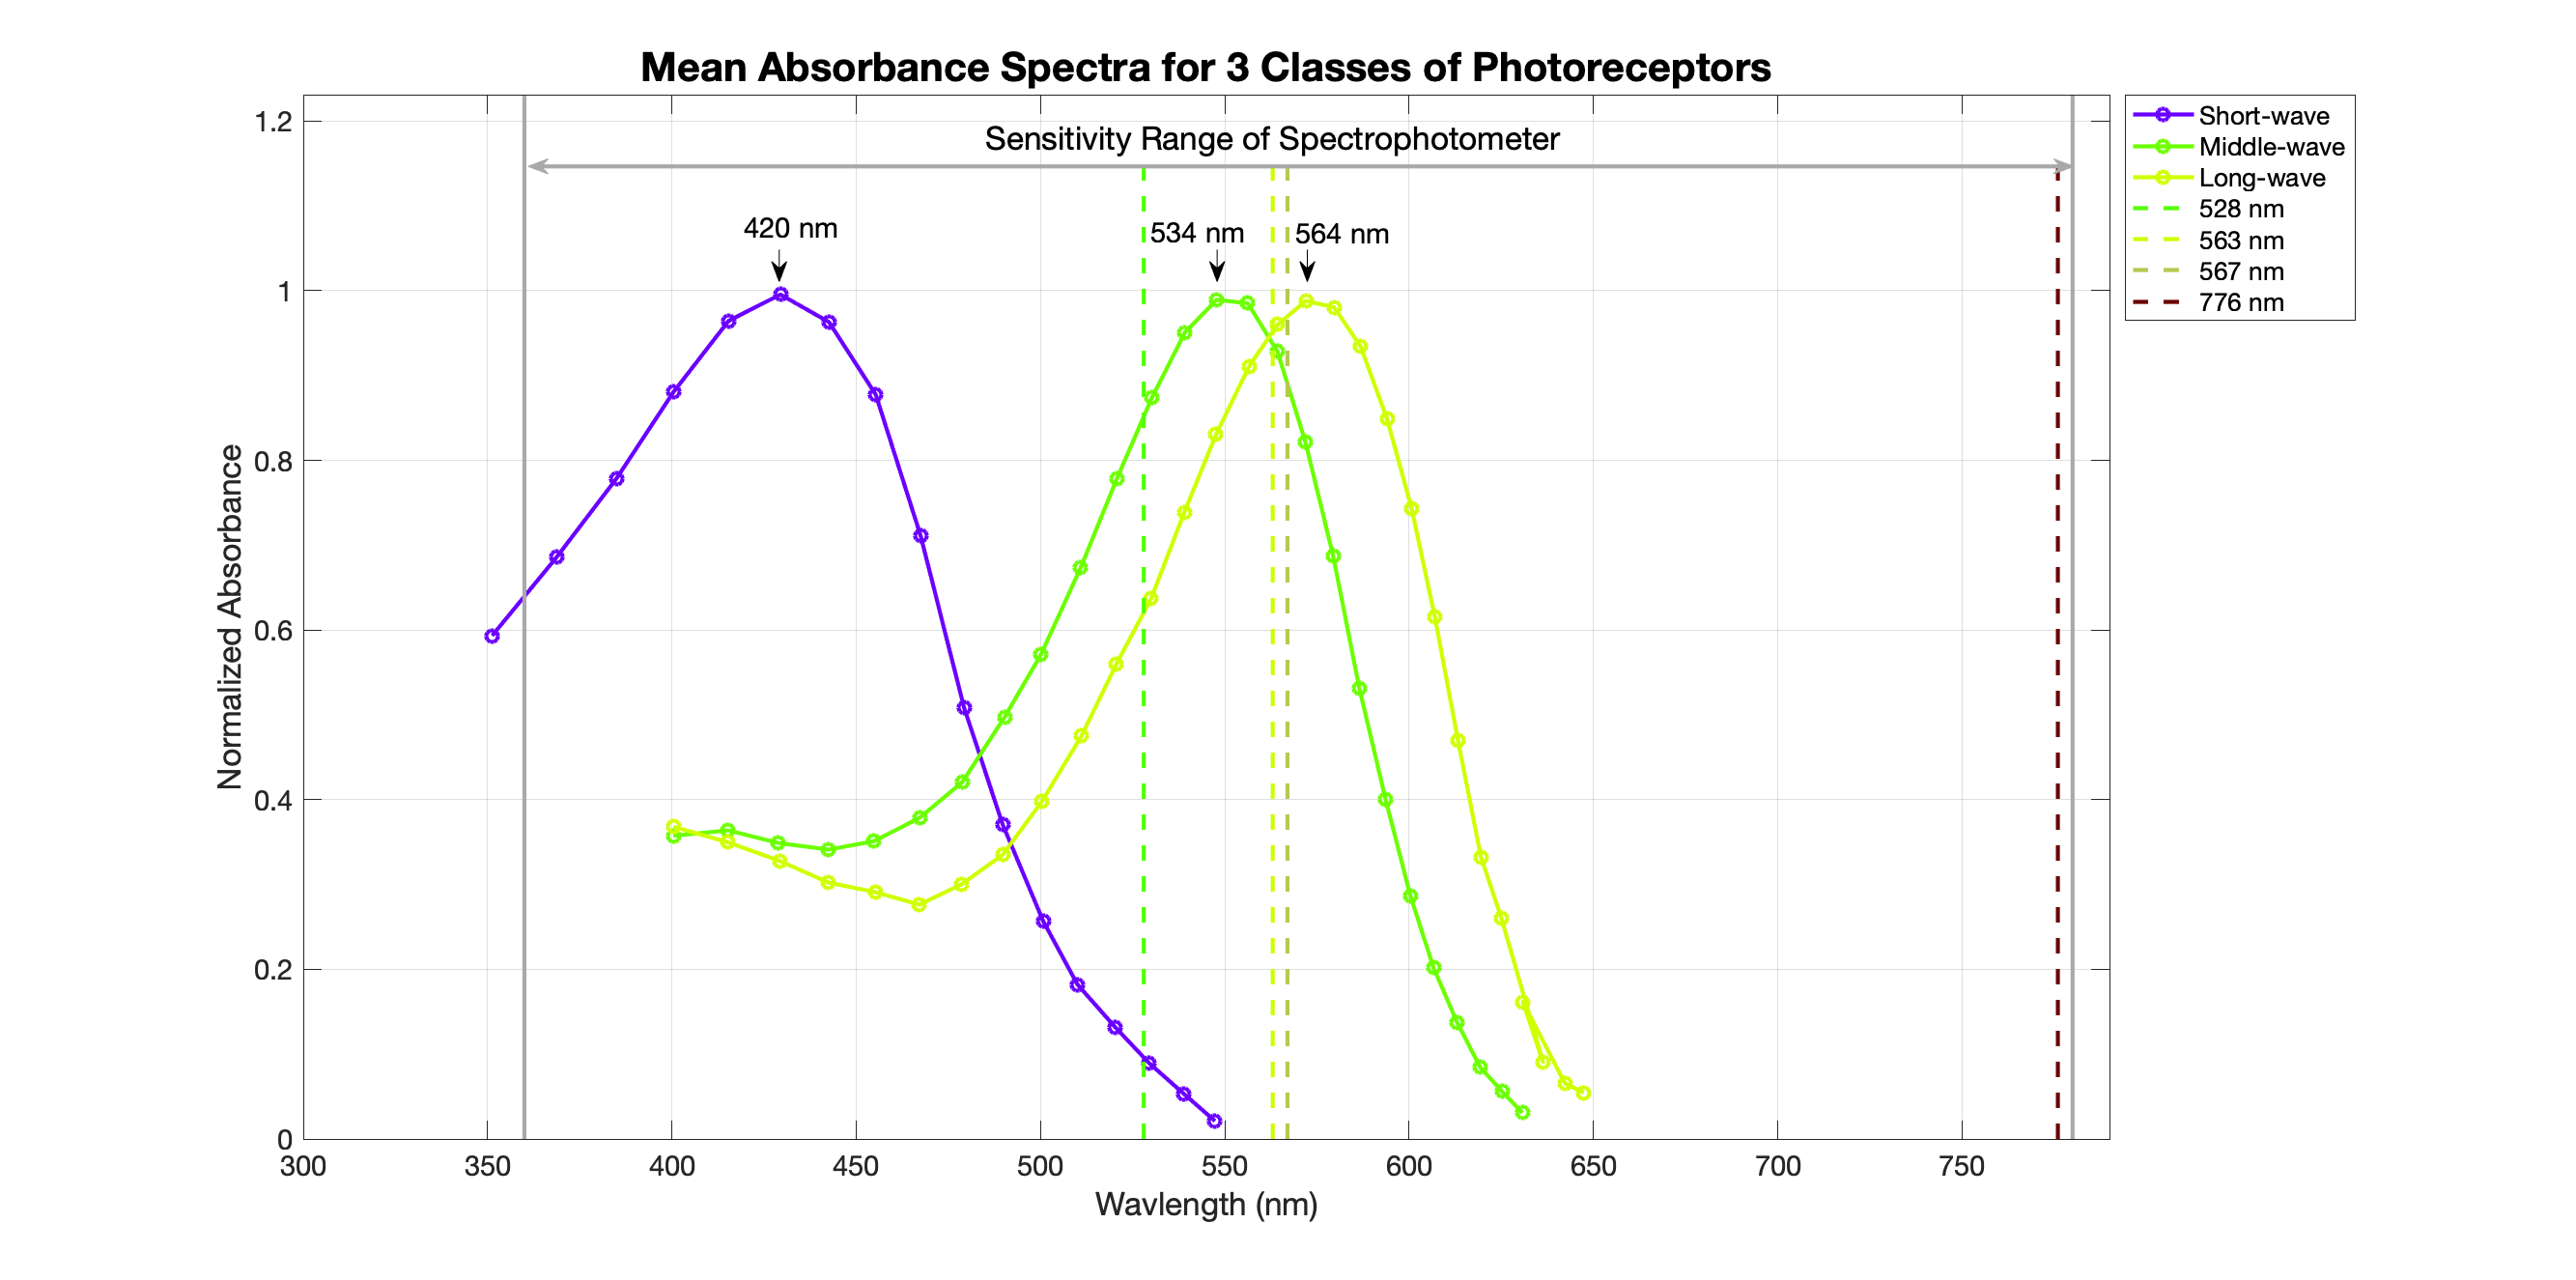
\includegraphics[width=0.95\textwidth]{./spectrum/AbsorbanceSpectra.png}
    
    \hspace{1.5in}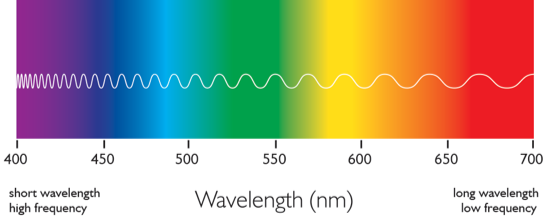
\includegraphics[width=0.425\textwidth]{./spectrum/light-spectrum.png}
    
    \caption{Normalized mean absorbance spectra for long-wave, middle-wave, and short-wave cones. Maximum absorbance values for each class of cones are 420 nm $\pm$ 4.7 nm, 534 nm $\pm$ 3.7 nm, and \hbox{564 $\pm$ 4.7 nm}, respectively. Dashed vertical lines represent the top 4 important predictors taken from the pupil diameter models created here. The sensitivity range of the Konica Minolta CL-500A Spectrophotometer is 360 -- 780 nm indicated by the gray double sided arrow. Cone absorbances were based on a figure in the  paper by Bowmaker and Dartnall \cite{BowmakerCones}}
    \label{fig:absorbances}
\end{figure}

New predictive empirical models of the pupil diameter can be derived using supervised multivariate non-linear non-parametric machine learning regression. The accuracy of the models can be evaluated using an independent validation (or testing) dataset whose data records were not utilized in the model training. This machine learning approach can also provide insights on the relative importance of the inputs (i.e. predictors). In this case we had a few hundred inputs, including the light intensities for every nm of wavelengths from 360 -- 780 nm (ultra-violet to near infrared). 

\section{Materials and Methods}

Data was collected during 3 outdoor/indoor walks where spectral and biometric data were recorded. The walks took place in the morning ($\approx$~8:30 AM) and late afternoons ($\approx$~4 PM), each lasting approximately fifteen minutes. Spectral data was measured approximately every 3 seconds using a NIST calibrated Konica Minolta CL-500A Illuminance Spectrophotometer, which measures the illuminance and spectral irradiance of wavelengths from 360 -- 780 nm with 1 $\pm$ 0.3 nm resolution. Pupil diameters, head orientation, and the proper acceleration of the head were recorded 100 times a second using Tobii Pro Glasses 2. The glasses use an infrared grid projected onto each eye to estimate the position and size of the pupils. The orientation and acceleration of the head are estimated using a microelectromechanical system (MEMS) gyroscope and MEMS accelerometer located in the glasses. Data was prepared and analyzed using Matlab 2019a. The data preparation involved six steps: 
\begin{enumerate}
    \item \textbf{Collection} - Recording of the raw data. Data was written to 6 separate files corresponding to the 2 devices for each of the 3 trials. 
    \item \textbf{Formatting} - Converting raw data files to Matlab timetable objects. 6 timetables were created from the raw data files.
    \item \textbf{Synchronizing} - The sampling frequencies differed for each device. 1 record every 3 seconds for the spectral data, versus 100 records every second for the biometric data. To account for this, the 2 timetables for a particular trial were reconfigured to share the same time steps using Matlab's \texttt{retime} function with a linear interpolation. The timetables for each trial could then combined using the \texttt{synchronize} function. Resulting in 3 timetables, one for each of the 3 trials. 
    \item \textbf{Merging} - Concatenating all 3 timetables into a single timetable. 
    \item \textbf{Cleaning} - Removing records with device error flags, NaN elements, and zero values for pupil diameter. The latter case is addressed below.
    \item \textbf{Generating} - Creating new variables such as the average pupil diameter and inter-eye pupil diameter difference.
\end{enumerate}

 \noindent A major challenge was introduced in step 5 (cleaning) of the data preparation due to a significant portion of the pupil diameter records taking values of 0. This was a non-physical consequence of the mechanism with which the pupil diameters were measured. When there is a high intensity of ambient infrared light from bright sunshine the glasses can no longer readily discern the pupil diameter, this is reflected in Figure \ref{fig:specPD} where pupil diameter dropouts coincide with time intervals of high spectral irradiance. These records were removed from the data, reducing the number of records from $\approx$ 380,000 to $\approx$ 80,000 records.
 
 \begin{figure}[!tbp]
    \centering
    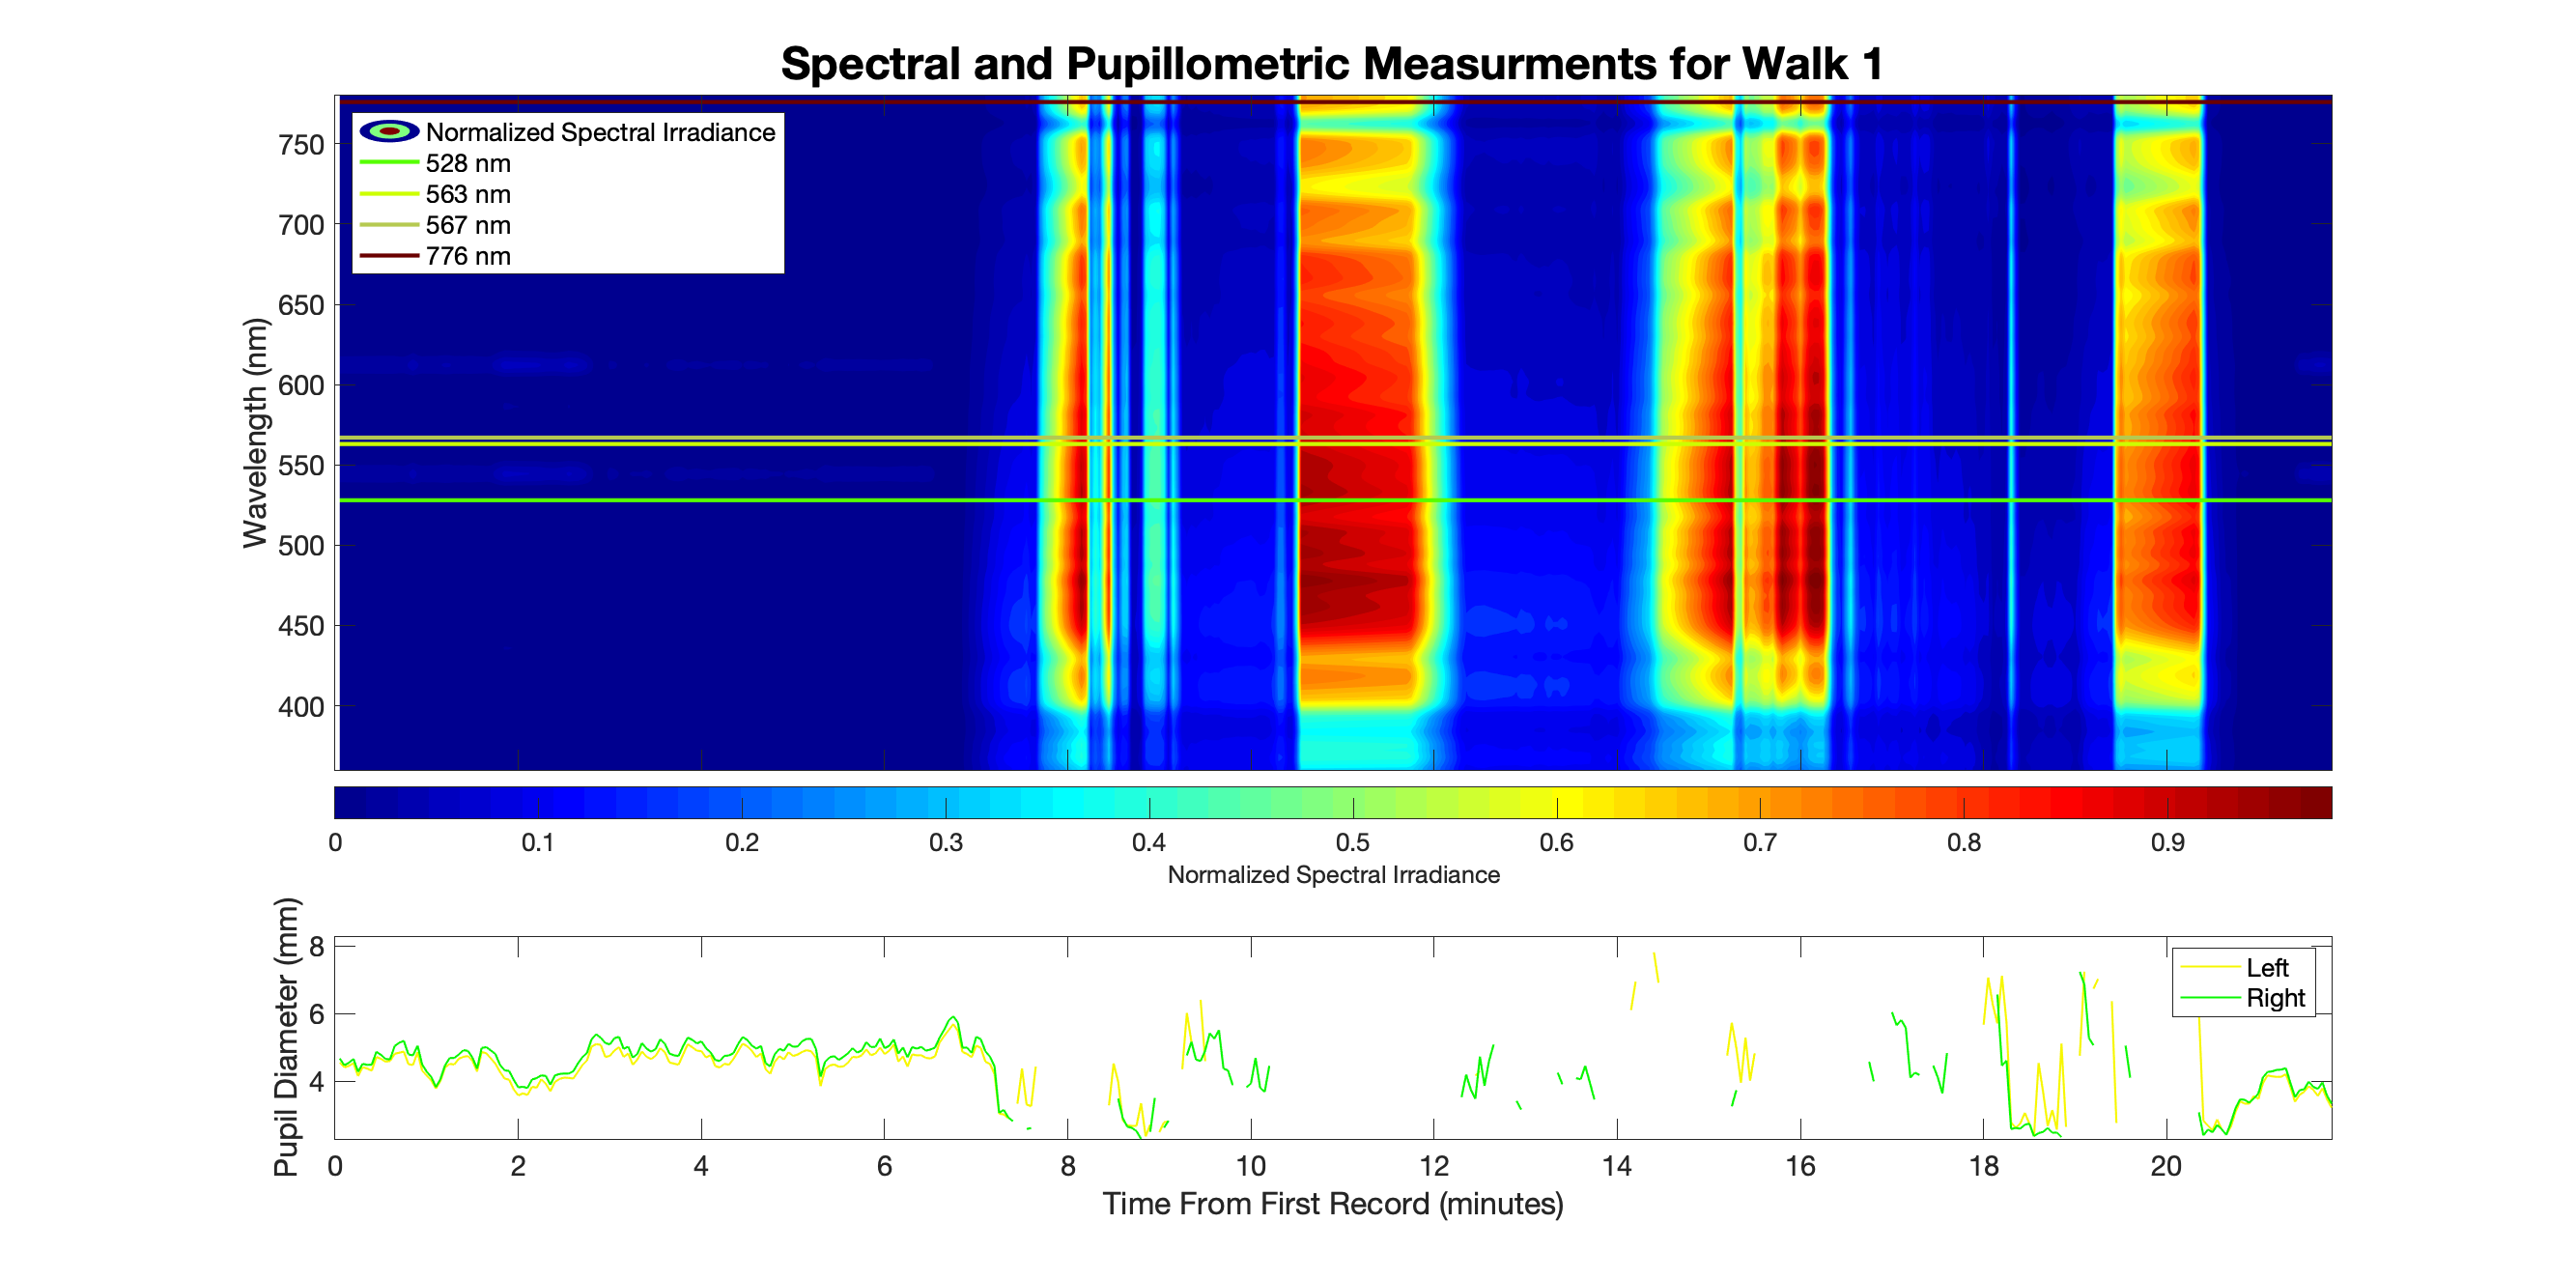
\includegraphics[width=0.85\textwidth, keepaspectratio]{./spectrum/spectrum3_2wPDRun1.png}
    
    \centering
    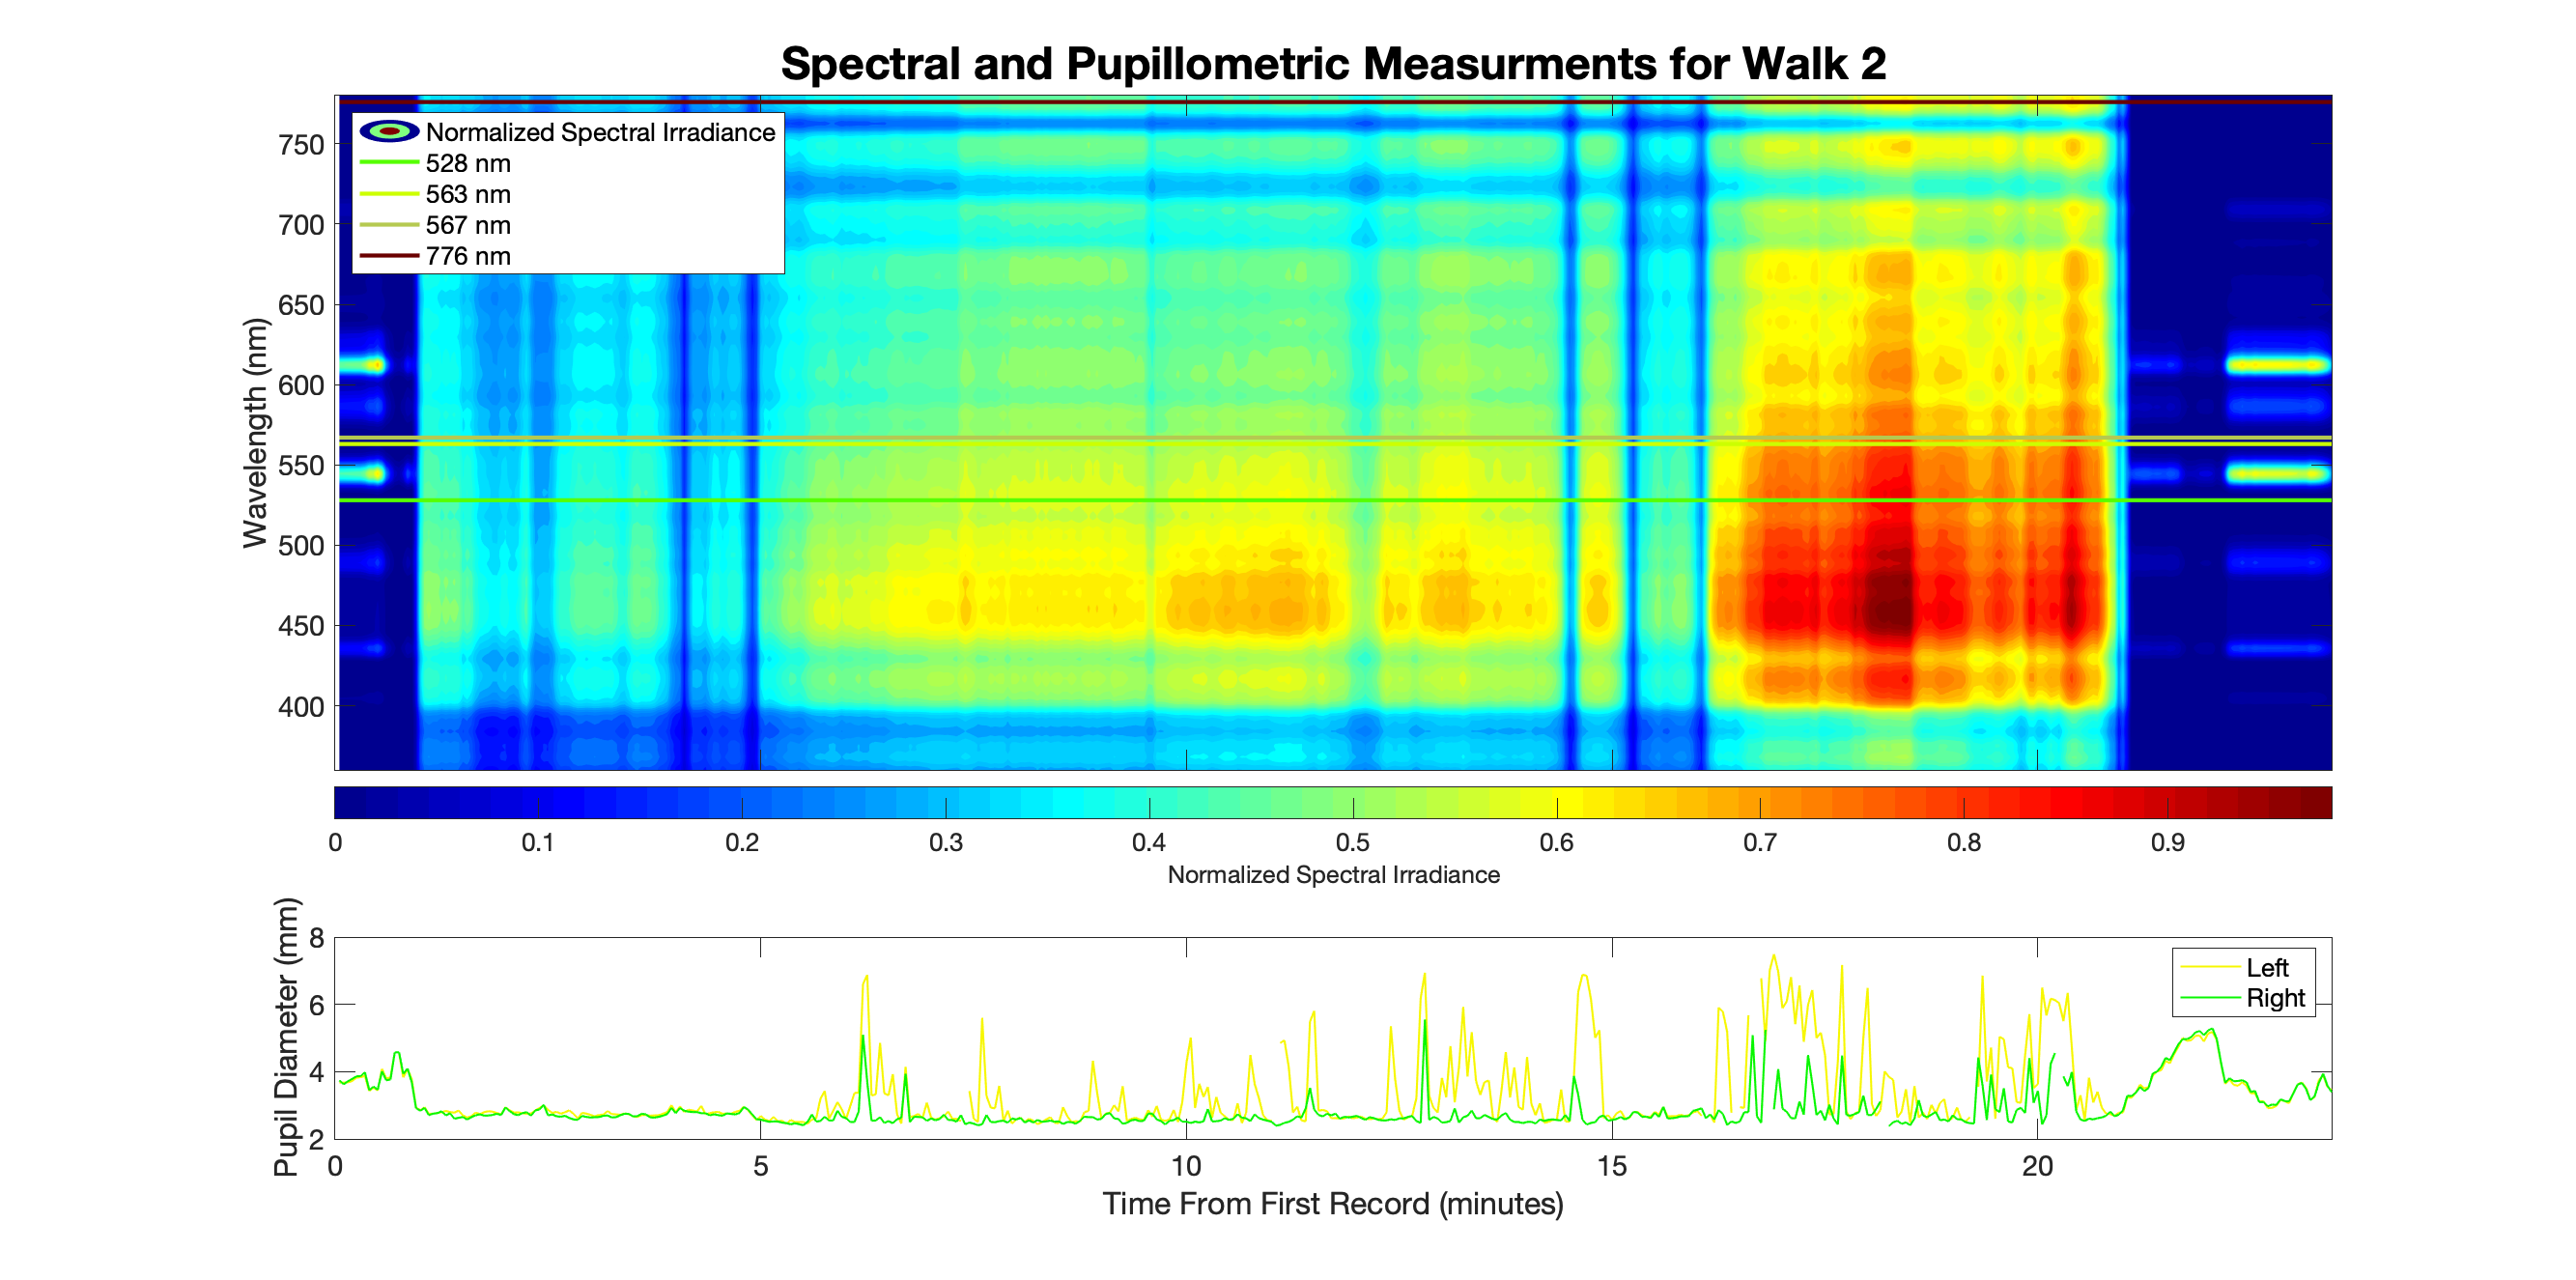
\includegraphics[width=0.85\textwidth, keepaspectratio]{./spectrum/spectrum3_2wPDRun2.png}
    
    \centering
    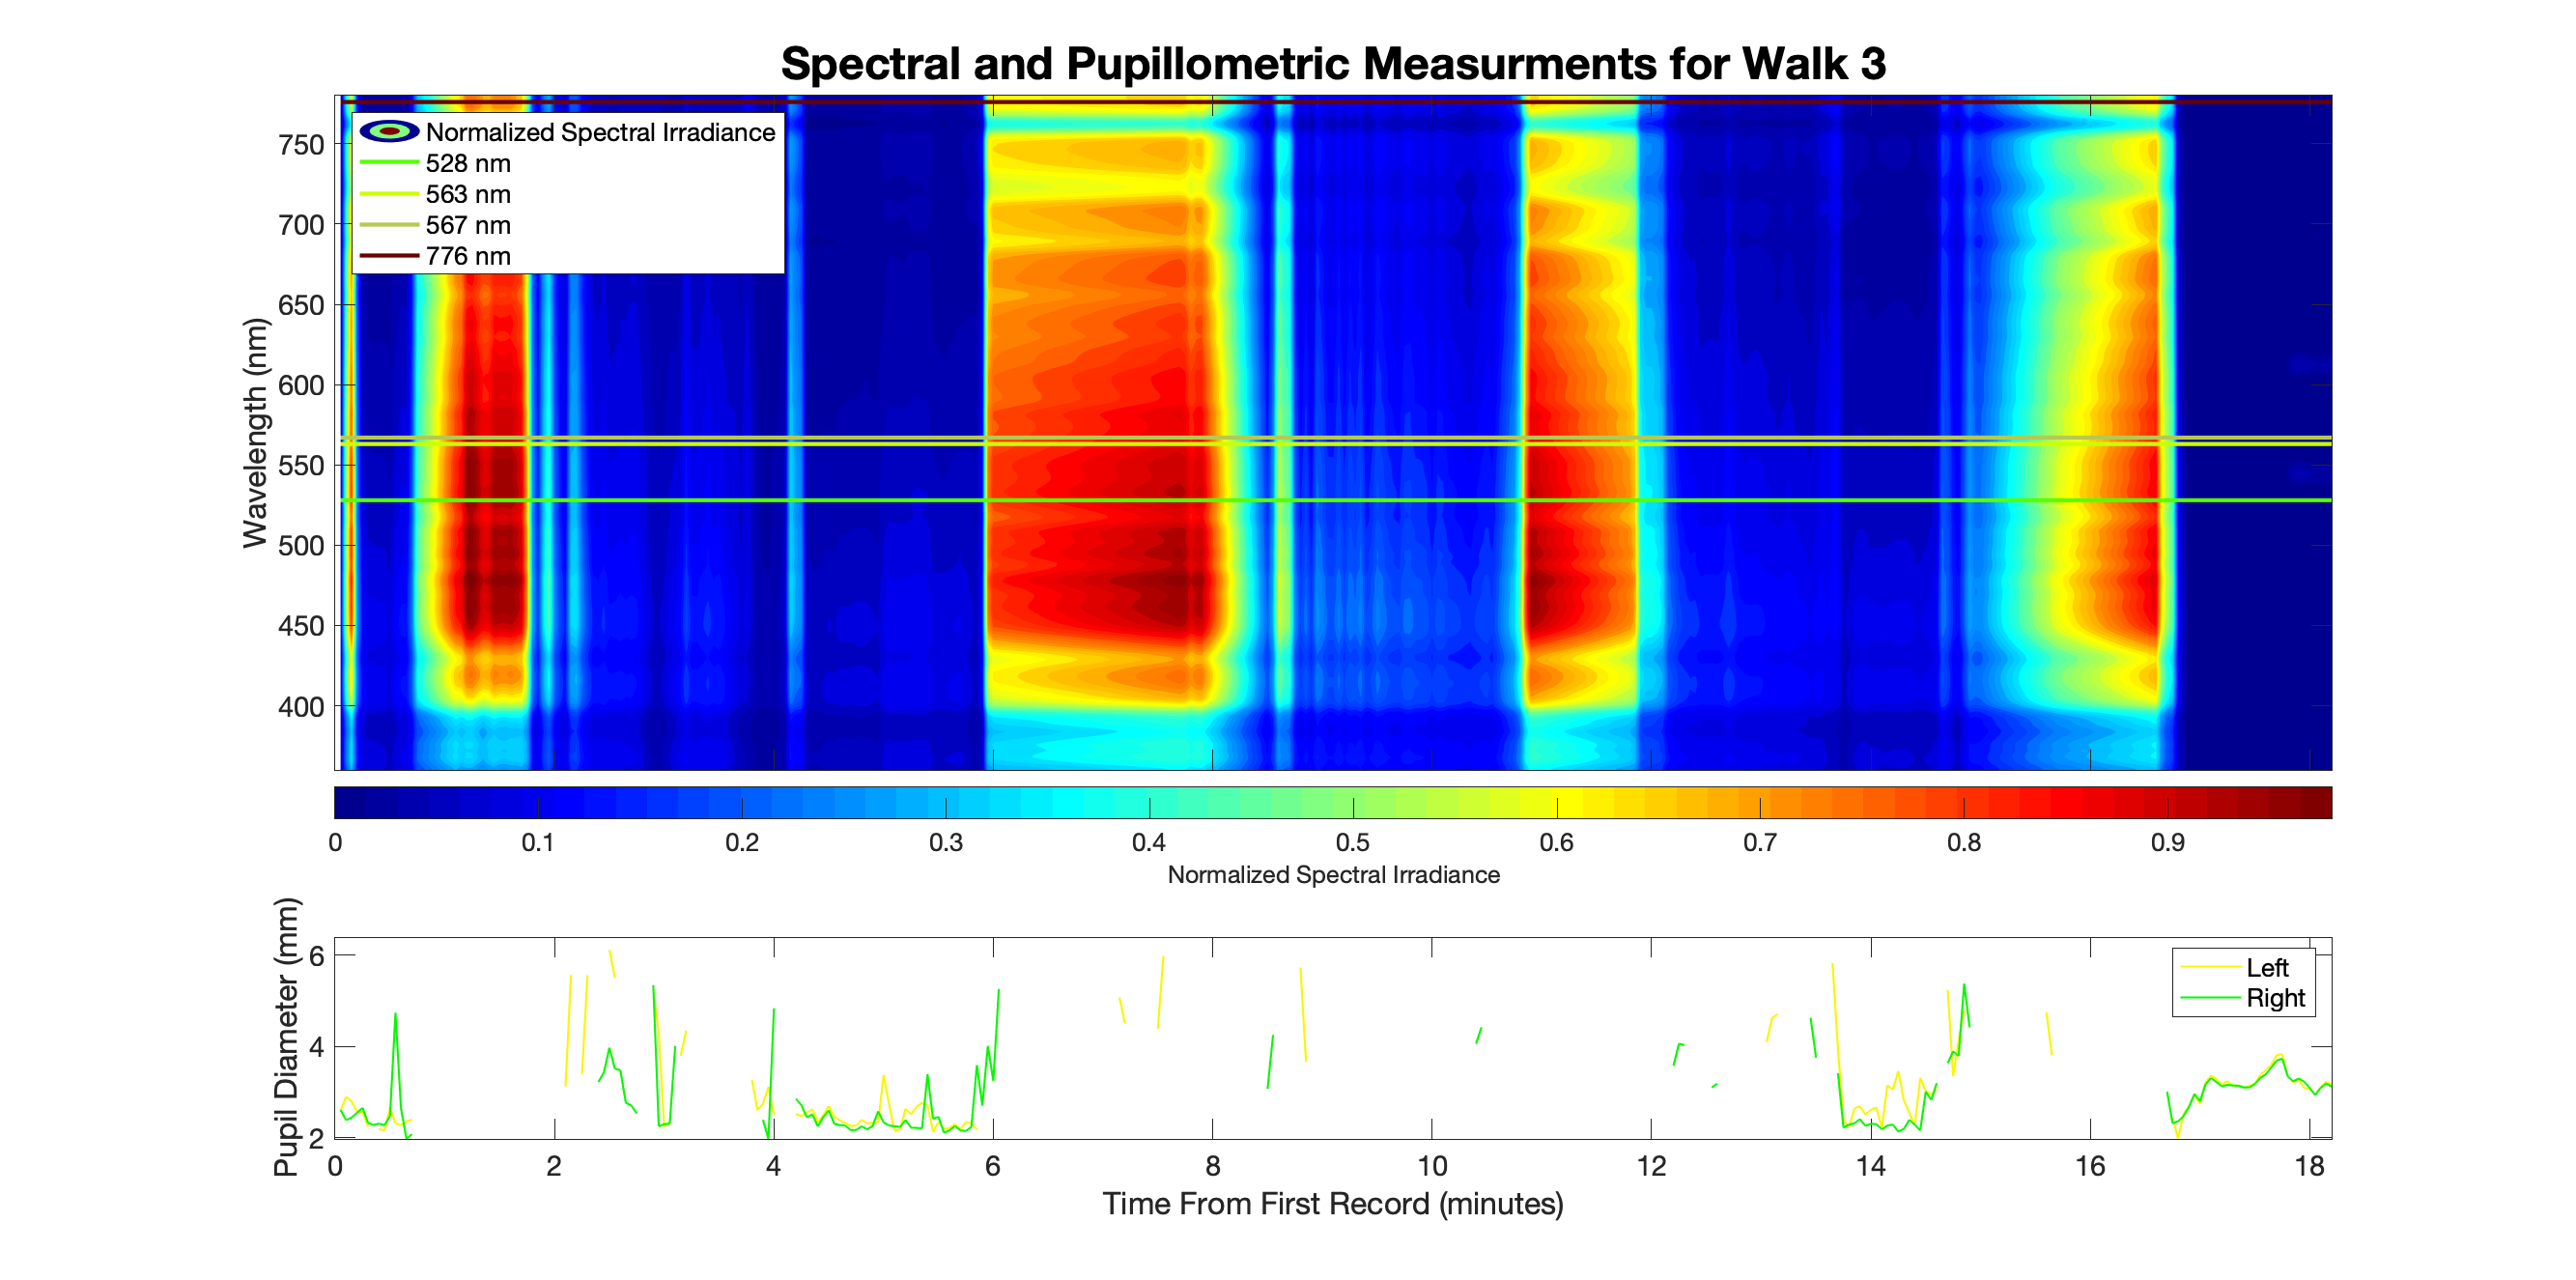
\includegraphics[width=0.85\textwidth, keepaspectratio]{./spectrum/spectrum3_2wPDRun3.png}
    
    \caption{The normalized spectral irradiance at every time step for all walks is plotted. The irradiance is normalized by dividing all values by the maximum spectral irradiance within each walk. Relative size of irradiance values are indicated by the colorbar. Spectral lines at 528, 563, 567, and 776 nm represent the most important predictors for the pupil diameter models. Left (yellow) and right (green) pupil diameters are plotted over time. Note the pupil diameter dropouts in time intervals where the spectral irradiance is high. (\textbf{a}) Walk 1 measurements during late afternoon ($\approx$ 4 PM). (\textbf{b}) Walk 2 measurements during morning ($\approx$ 8:30 AM) with overcast. (\textbf{c}) Walk 3 measurements during late afternoon ($\approx$ 4 PM).}
    
    \label{fig:specPD}
\end{figure}
 
 From the recorded data we sought to estimate 5 different parameters, namely the: average of the left and right pupil diameters (APD), left pupil diameter (LPD), right pupil diameter (RPD), magnitude of the difference between the left and right pupil diameters (PDD), and the illuminance. These parameters can be estimated by constructing objectively optimized empirical machine learning models. The hyperparameters (i.e. the parameters that define options associated with the training process) of an ensemble of regression trees able to use both boosting and bagging were optimized (the Matlab function  \texttt{fitrensemble} with the \texttt{OptimizeHyperparameters} option set to \texttt{all}). More information on this function is available in the Matlab documentation \cite{Matlab}. We have done many previous machine learning studies \cite{lary2016machine, brown2008neural, lary2009machine, lary2008space, lary2004using, malakar2013towards, lary2010artificial, malakar2012estimation, lary2013using, lary2007using, albayrak2011modis, brown2006using, lary2003using, malakar2012towards, lary2014bigdata, lary2015using, kneen2016interpretation, lary2010machine, medvedev2016analysis, lary2016using, o2017demonstration, wu2017insights, nathan2019combining, lary2019using, lary2018machine, wu2019using, alavi2016progress, ahmad2016devices, zewdie2018applying, malakar2018case, zewdie2019applying, zewdie2019estimating, chang2019time}.

The data was split into 2 subsets: one for training and one for the independent testing of each empirical machine learning model. With 90\% of the data used for training the multivariate non-linear non-parametric regression models and 10\% of the data used for independent testing of the models. 

% Five separate models were created using different combinations of inputs for the pupil diameter of the left eye, the right eye, and the average pupil diameter of both eyes, using the spectral illuminance measured every nm between 360 and 780 nm, the gyroscope, and the accelerometer data as predictor variables. A fourth model assessed the pupil asymmetry by modeling the pupil diameter difference with the same predictor variables as before. Further assessment of the pupil asymmetry was considered by applying the model for the left pupil diameter to predict the right pupil diameter and vice versa. Finally, a model was trained to test whether the illuminance could be predicted from the pupil diameters, gyroscope, and accelerometer data. 

All the data and code used in this study is publicly available at the LightOcular GitHub repository: \url{https://github.com/mi3nts/LightOcular}. All the data used in this study is also publicly available as a Zenodo data store: \url{https://zenodo.org/record/3354602#.XUi9wJNKjVp}, doi: 10.5281/zenodo.3354602.

\section{Results and Discussion}

In the following subsections we discuss the results of the 5 different empirical machine learning models. The accuracy of each model was assessed via a scatter plot of the true vs estimated response variable values (see Figures \ref{fig:APD}a, \ref{fig:LPD}a, \ref{fig:RPD}a, \ref{fig:PDD}a, \& \ref{fig:ILM}a). If the true and estimated values are identical, the resulting scatter plot will be a straight line with a slope of one and an intercept of zero, i.e. a perfect one to one plot with a correlation coefficient, r$^{2}$, equal to 1. This ideal is indicated by a black line in each scatter plot. The correlation coefficients for the training (plotted as green circles) and testing (plotted as red pluses) datasets were computed using Matlab's \texttt{corrcoef} function.

The relative predictor importance ranking of each model was derived using the \texttt{predictorImportance} function. The relative rankings are visualized as bar plots (see Figures \ref{fig:APD}b, \ref{fig:LPD}b, \ref{fig:RPD}b, \ref{fig:PDD}b, \& \ref{fig:ILM}b). The importance estimates are plotted on a log scale with the most important predictors shown toward the top. In the pupil diameter models (i.e. models for the APD, LPD, RPD, and PDD), the top 20 out of 427 predictors are shown. For the illuminance model, all 7 predictors are given in the ranking. The top 3 predictors are indicated by red bars, the next 2 important predictors by yellow bars, and the remaining predictors by blue bars.

\subsection{The Average Pupil Diameter Model}

Figure \ref{fig:APD} shows the results of the average pupil diameter (APD) model. The APD was estimated using the spectral irradiance at every nm between 360 -- 780 nm, the gyroscope, and the accelerometer data as predictor variables. The scatter plot of the true vs the estimated average pupil diameter values is shown in Figure \ref{fig:APD}a. The model had correlation coefficients of $>$ 0.99 for both the training and testing data subsets. Thus, the empirical machine learning model was successful in predicting the average pupil diameter. Figure \ref{fig:APDb} shows the ranking of the relative importance of the inputs in predicting the APD, the top 3 predictors are the irradiance values at 561, 563, and 562 nm, which coincides with the maximum absorbance of the long-wave cones at around 563 nm \cite{BowmakerCones}. This suggests the long-wave photo-receptors play a more significant role than the short- or middle-wave receptors in controlling the average size of the pupils for the participant.

\begin{figure}[!b]
  \centering
  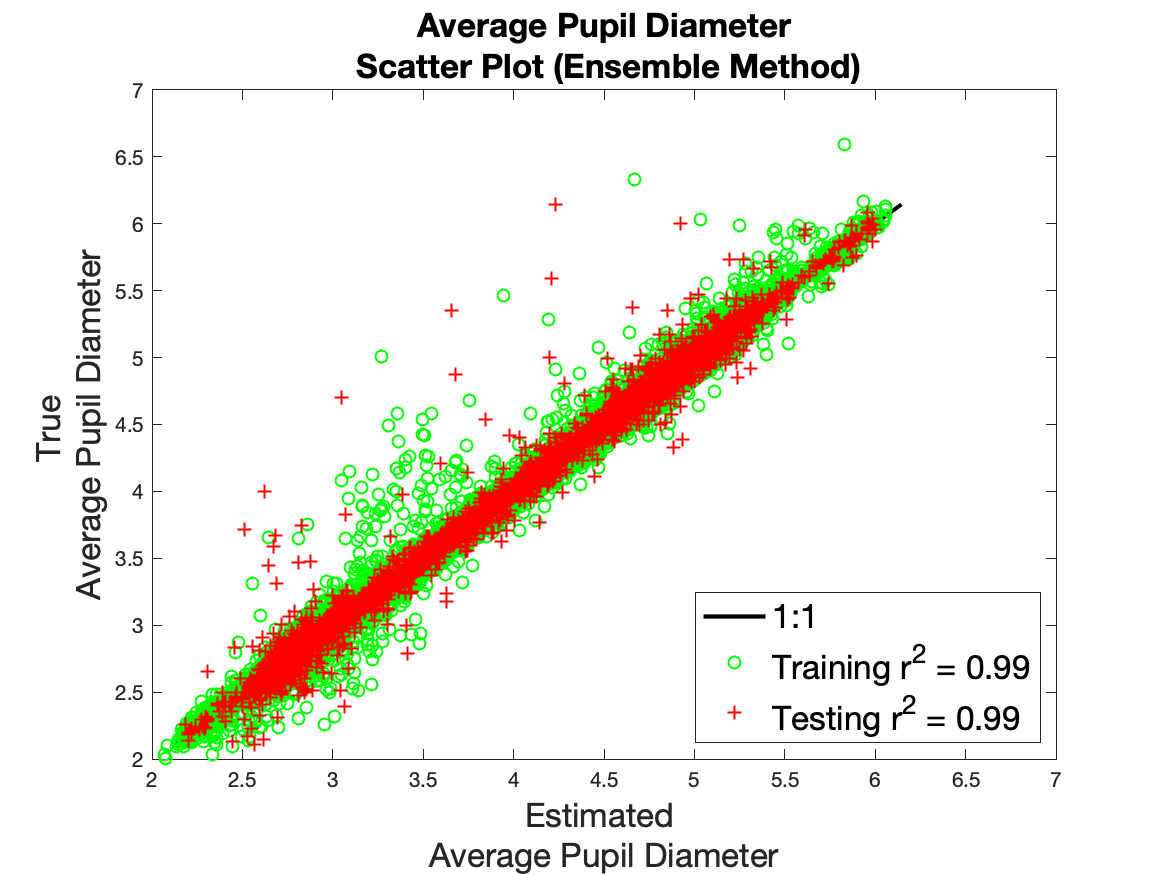
\includegraphics[width=0.48\textwidth]{./scatterPlots/AveragePupilDiameter_Ensemble_Scatter2.png}\label{fig:APDa}
  \hfill
  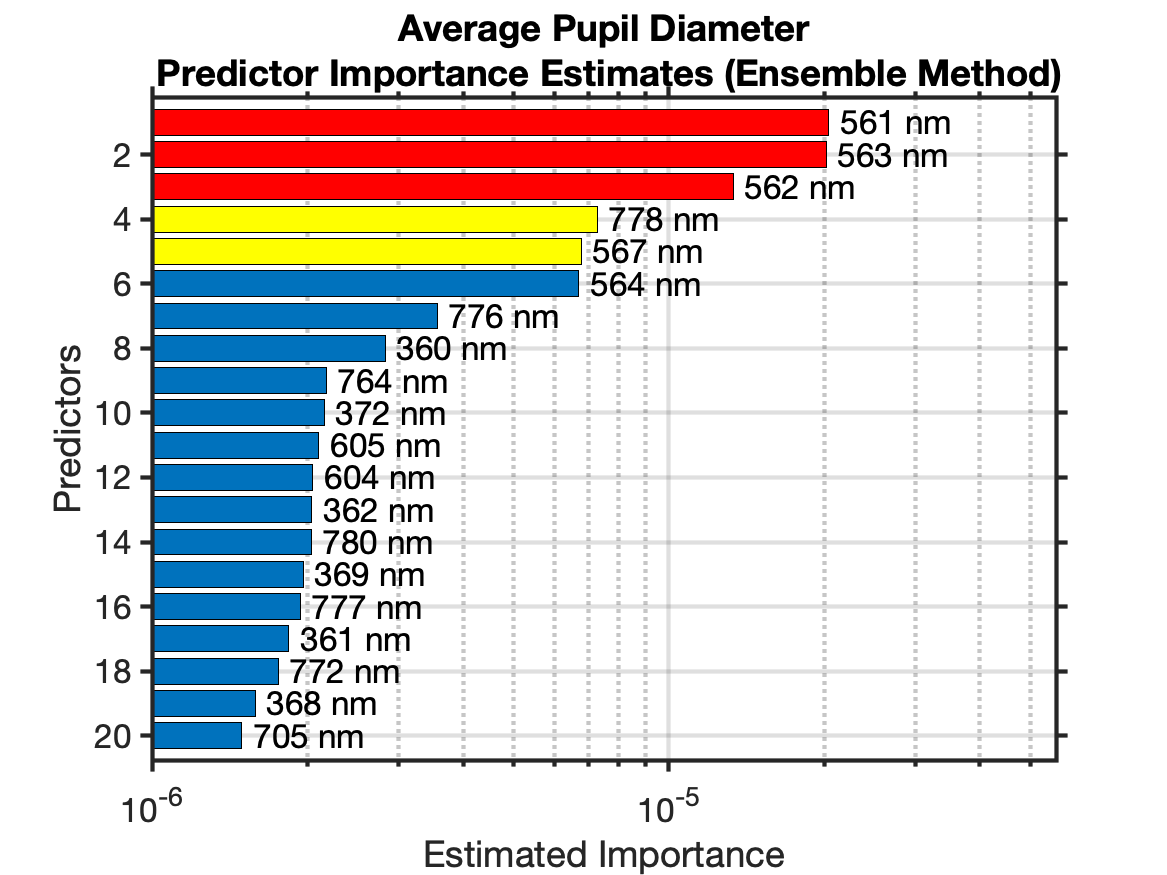
\includegraphics[width=0.48\textwidth]{./importanceRankings/AveragePupilDiameterEnsembleImpRankT20.png}\label{fig:APDb}
  \caption{Plots for the average pupil diameter model. (\textbf{a}) True vs estimated average pupil diameter in millimeters. (\textbf{b}) Predictor importance estimates for the average pupil diameter model.
  }
  \label{fig:APD}
\end{figure}

\subsection{The Left Pupil Diameter Model}

The results for the left pupil diameter (LPD) model are shown in Figure \ref{fig:LPD}. The LPD was estimated using the same predictors as the APD, the spectral irradiance from 360 -- 780 nm, the gyroscope, and the accelerometer data. The model was successful in predicting the LPD with a correlation coefficient of \hbox{$>$ 0.96} for both the training and validation data subsets. The top predictor (\hbox{567 nm}) is again near the maximum absorbance of the long-wave photo-receptors (\hbox{563 nm}). The next top 6 predictors are the irradiance values at 528, 568, 564, 527, 668, and 570 nm, which seem to coincide with both the middle and long-wave photo-receptors with maximum absorbance values near 533.8 $\pm$ 3.7 nm and 563 nm, respectively, with the exception of the irradiance at 668 nm \cite{BowmakerCones}.

\begin{figure}[!b]
  \centering
  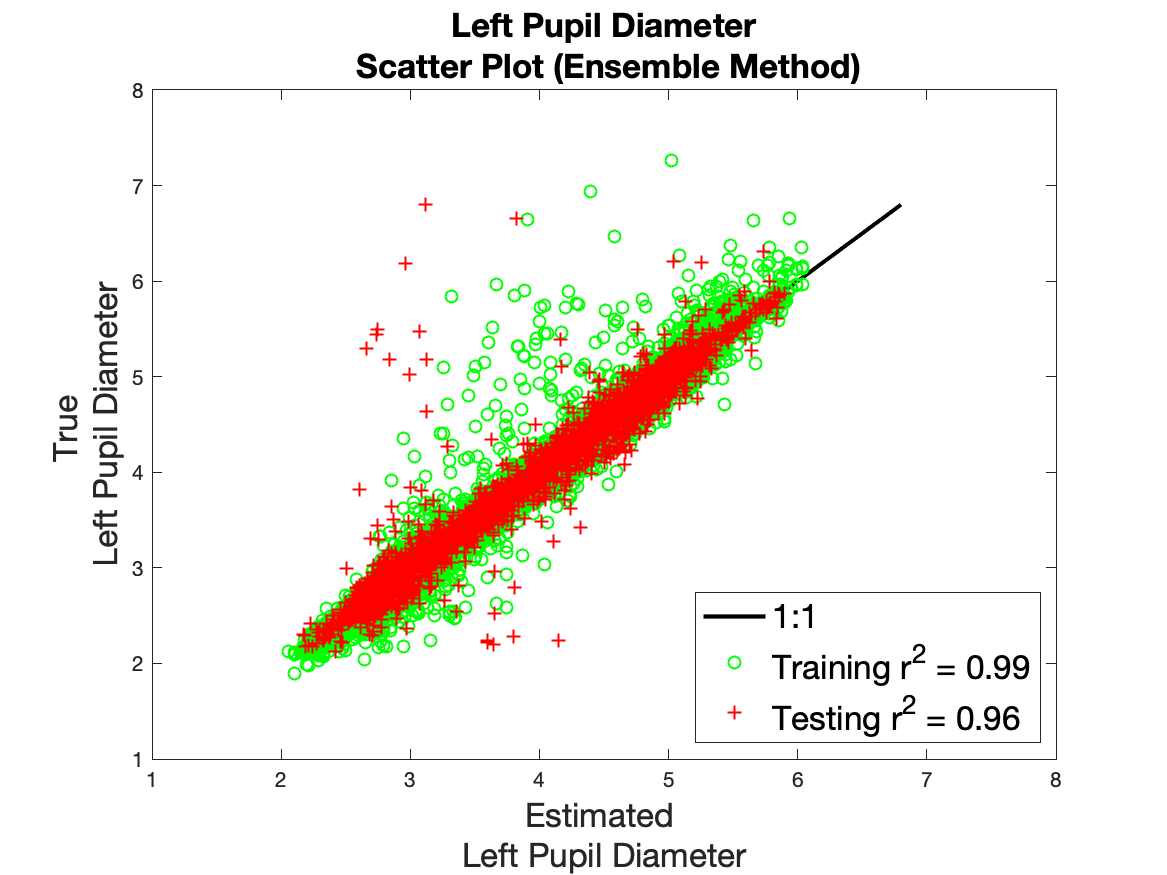
\includegraphics[width=0.48\textwidth]{./scatterPlots/LeftPupilDiameter_Ensemble_Scatter2.png}\label{fig:LPDa}
  \hfill
  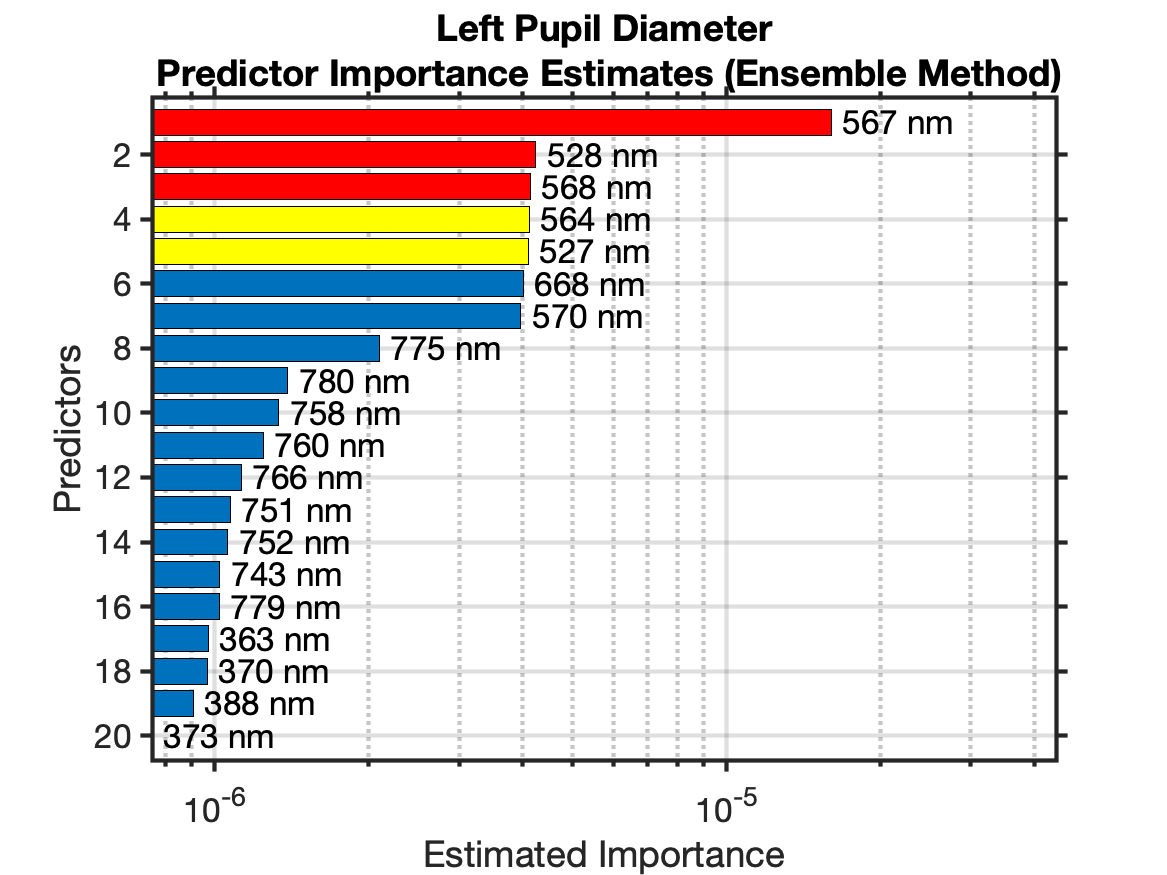
\includegraphics[width=0.48\textwidth]{./importanceRankings/LeftPupilDiameterEnsembleImpRankT20.png}\label{fig:LPDb}
  \caption{Plots for the left pupil diameter model. (\textbf{a}) True vs estimated left pupil diameter in millimeters. (\textbf{b}) Predictor importance estimates for the left pupil diameter model.
  \label{fig:LPD}
  }
\end{figure}

\subsection{The Right Pupil Diameter Model}

The results for the right pupil diameter (RPD) model are shown in Figure \ref{fig:RPD}. The RPD was estimated using the same predictors as the APD and LPD. For the RPD model there is a strong correlation between the estimated and true values, with coefficients of determination $>$ 0.99 for both data subsets, shown in Figure \ref{fig:RPD}a. The top 2 predictors are 563 nm and 562 nm, which again coincide with the maximum absorbance of the long-wave cones near 563 nm. The next most important predictor was the irradiance at 776 nm corresponding to near infrared light. This and the appearance of near infrared predictors in all the importance rankings may be a consequence of the infrared noise in the environment, resulting in the measured pupil diameters to be smaller than the actual values. An interesting result from the importance ranking in Figure \ref{fig:RPD}b, is the appearance of a non-spectral predictor (Accelerometer Z) which denotes the proper acceleration in the direction in front of the glasses. This may be correlated to the participant looking down to navigate obstacles in the walking path such as stairs, inclines, rugged terrain, and other impediments. Focusing on a specific task or object may cause an increase in cognitive load, resulting in a pupillary response \cite{PupilLoad3,PupilLoad4}.

\begin{figure}[!t]
  \centering
  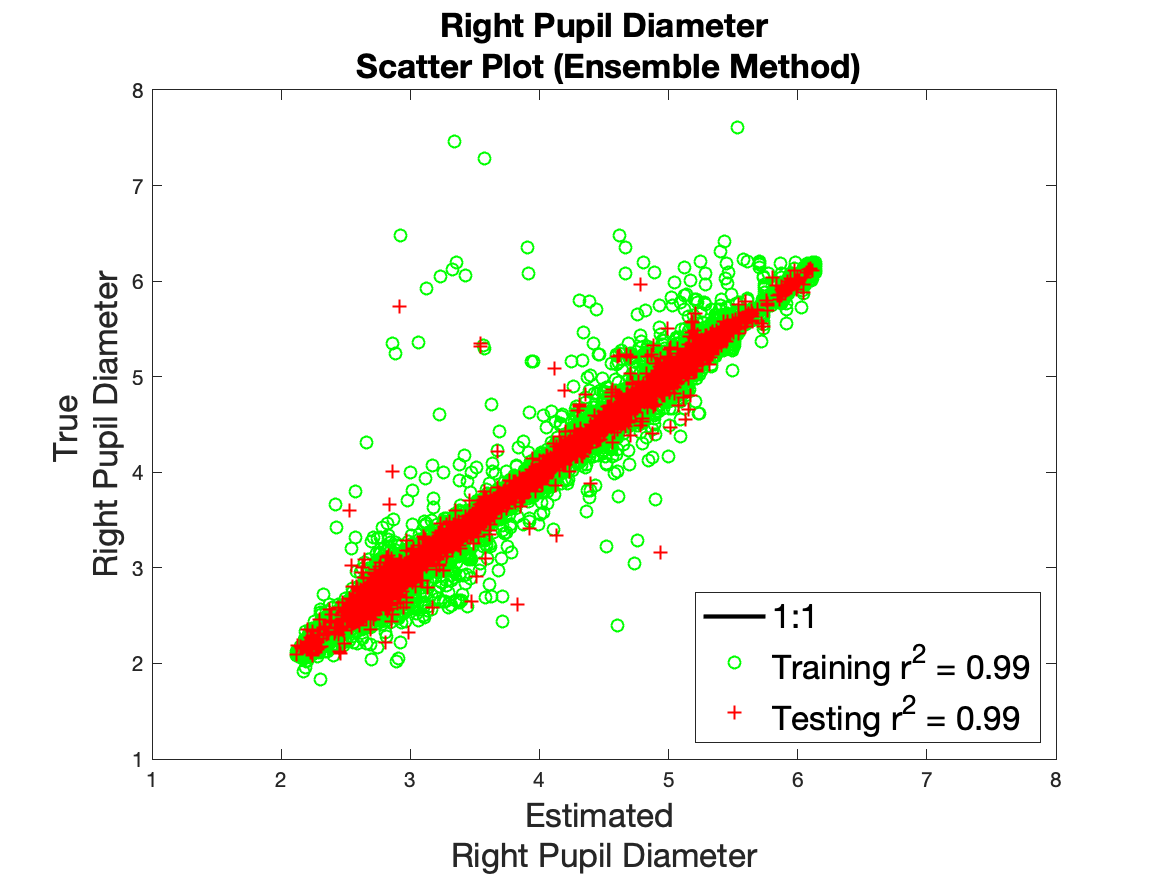
\includegraphics[width=0.48\textwidth]{./scatterPlots/RightPupilDiameter_Ensemble_Scatter2.png}\label{fig:RPDa}
  \hfill
  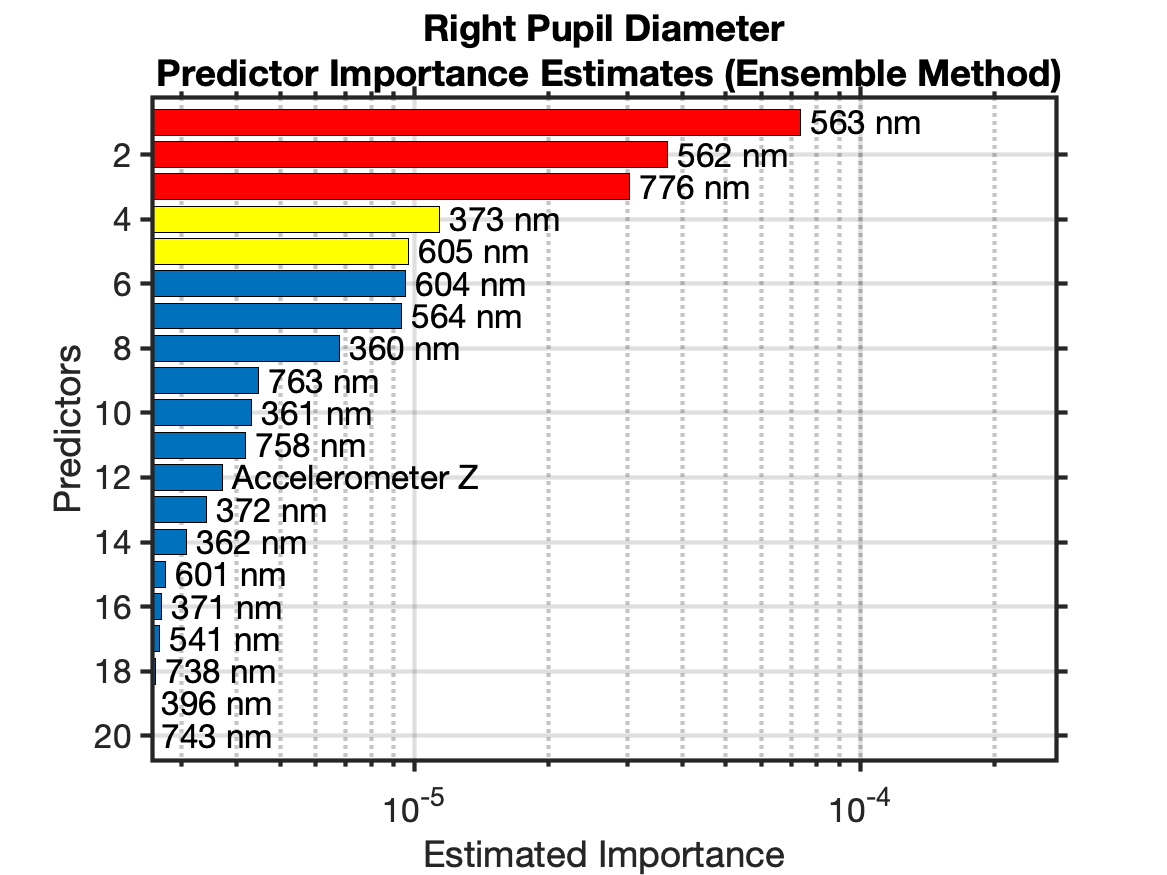
\includegraphics[width=0.48\textwidth]{./importanceRankings/RightPupilDiameterEnsembleImpRankT20.png}\label{fig:RPDb}
  \caption{Plots for the right pupil diameter model in millimeters. (\textbf{a}) True vs estimated right pupil diameter. (\textbf{b}) Predictor importance estimates for the right pupil diameter model.
  }
  \label{fig:RPD}
\end{figure}

\subsection{The Pupil Diameter Difference Model and Pupil Asymmetry}

The results for the left and right pupil diameter models are noticeably different (see Figures \ref{fig:LPD} and \ref{fig:RPD}), which may suggest an asymmetry in the behavior of each pupil. One measure of this asymmetry is the magnitude of the difference between the left and right pupil diameters. This is shown by the results of the pupil diameter difference (PDD) model given in Figure \ref{fig:PDD}. The same predictors were used for the PDD model as in the APD, LPD, and RPD models. This empirical model was not successful in predicting the PDD, since the correlation coefficient was 0.43 for the testing data subset, as shown in \ref{fig:PDDa}. Clearly the most important predictors for modeling this asymmetry were not available in the training dataset. 

Another metric of the pupil asymmetry can be the accuracy of the LPD model in estimating the RPD and vice versa. The resulting scatter plots are given in Figure \ref{fig:OPM}. Despite the differences in the importance rankings and failures of the PDD model, the estimates are fairly accurate with correlation coefficients of $>$ 0.95 for both the testing and training datasets. This accuracy may suggest that although there is an asymmetry in the importance rankings for the left and right pupil models, the functioning of each pupil is very similar. A possible cause of this asymmetry is ocular dominance (i.e. the input for one eye is preferred over the other) \cite{OcularDom1, OcularDom2}. It has been suggested that ocular dominance is not a static phenomenon, but will vary with changing horizontal gaze angle \cite{OcularDomAngle}. 

\begin{figure}[!t]
  \centering
  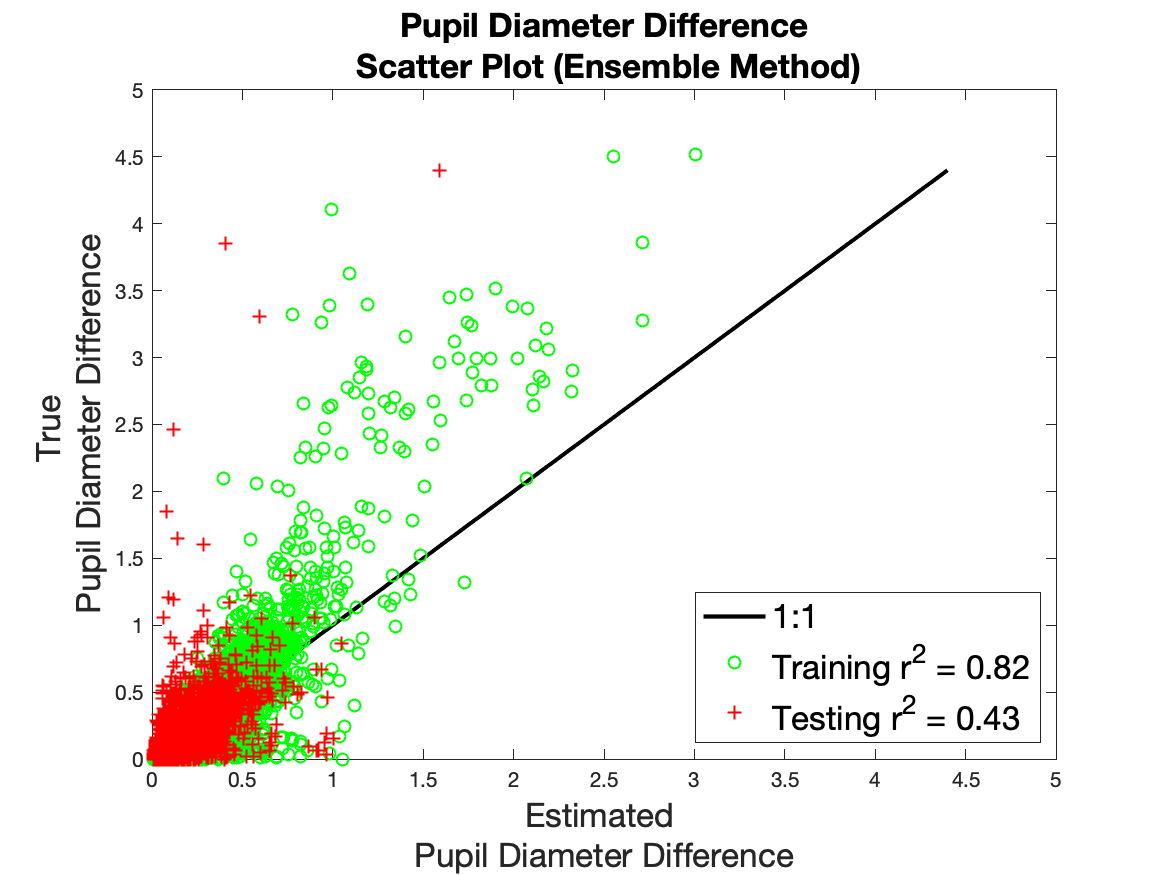
\includegraphics[width=0.48\textwidth]{./scatterPlots/PupilDiameterDifference_Ensemble_Scatter2.png}\label{fig:PDDa}
  \hfill
  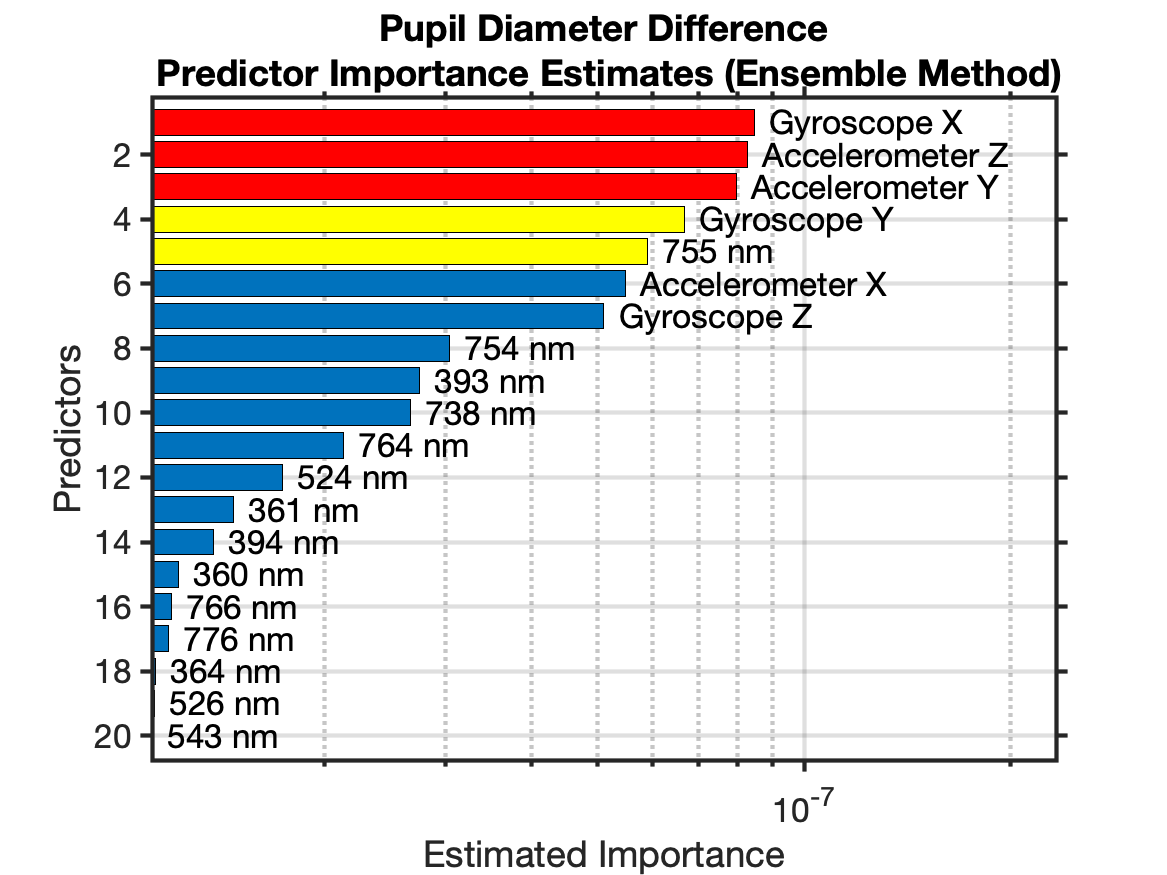
\includegraphics[width=0.48\textwidth]{./importanceRankings/PupilDiameterDifferenceEnsembleImpRankT20.png}\label{fig:PDDb}
  \caption{Plots for the pupil diameter difference model. (\textbf{a}) True vs estimated pupil diameter differences in millimeters. (\textbf{b}) Predictor importance estimates for the pupil diameter difference model.
  }
  \label{fig:PDD}
\end{figure}

\begin{figure}[!t]
  \centering
  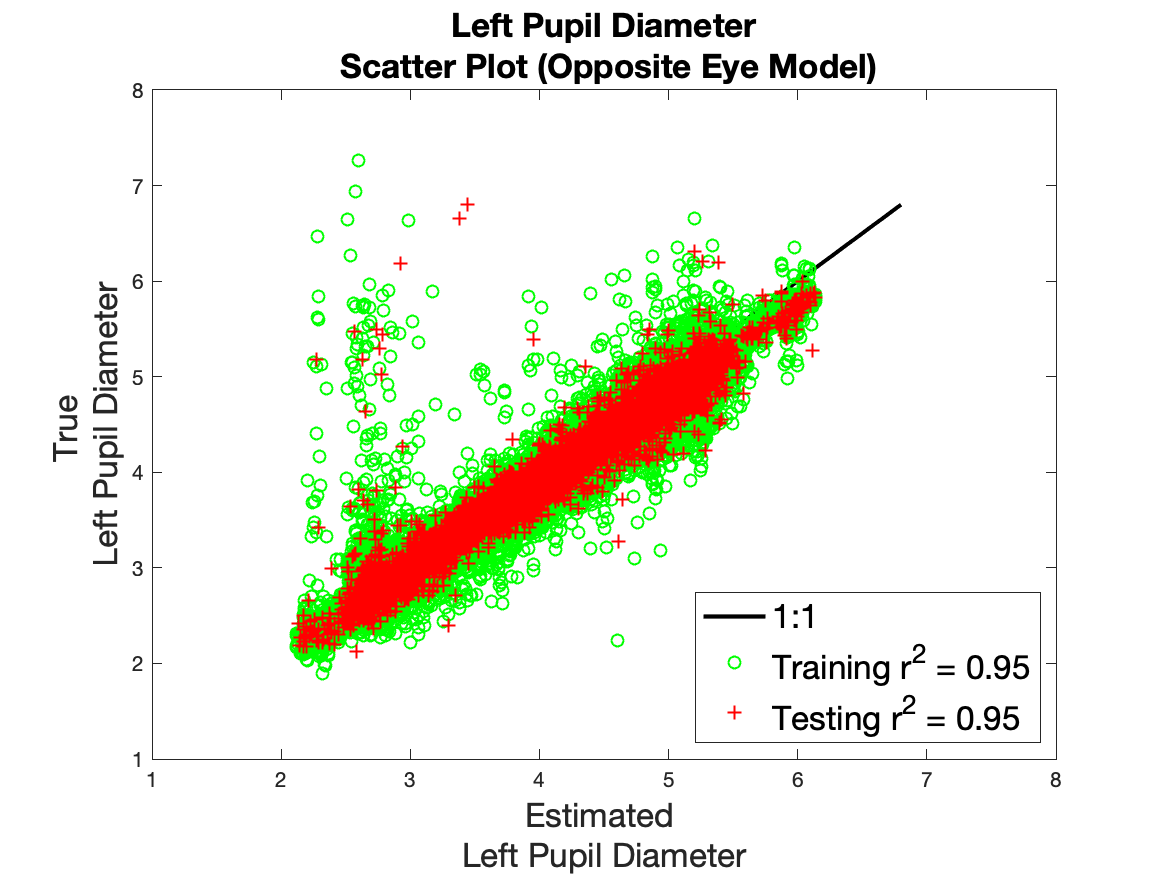
\includegraphics[width=0.48\textwidth]{./scatterPlots/LeftPupilDiameter_Ensemble_oppMdl_Scatter2.png}\label{fig:OPMa}
  \hfill
  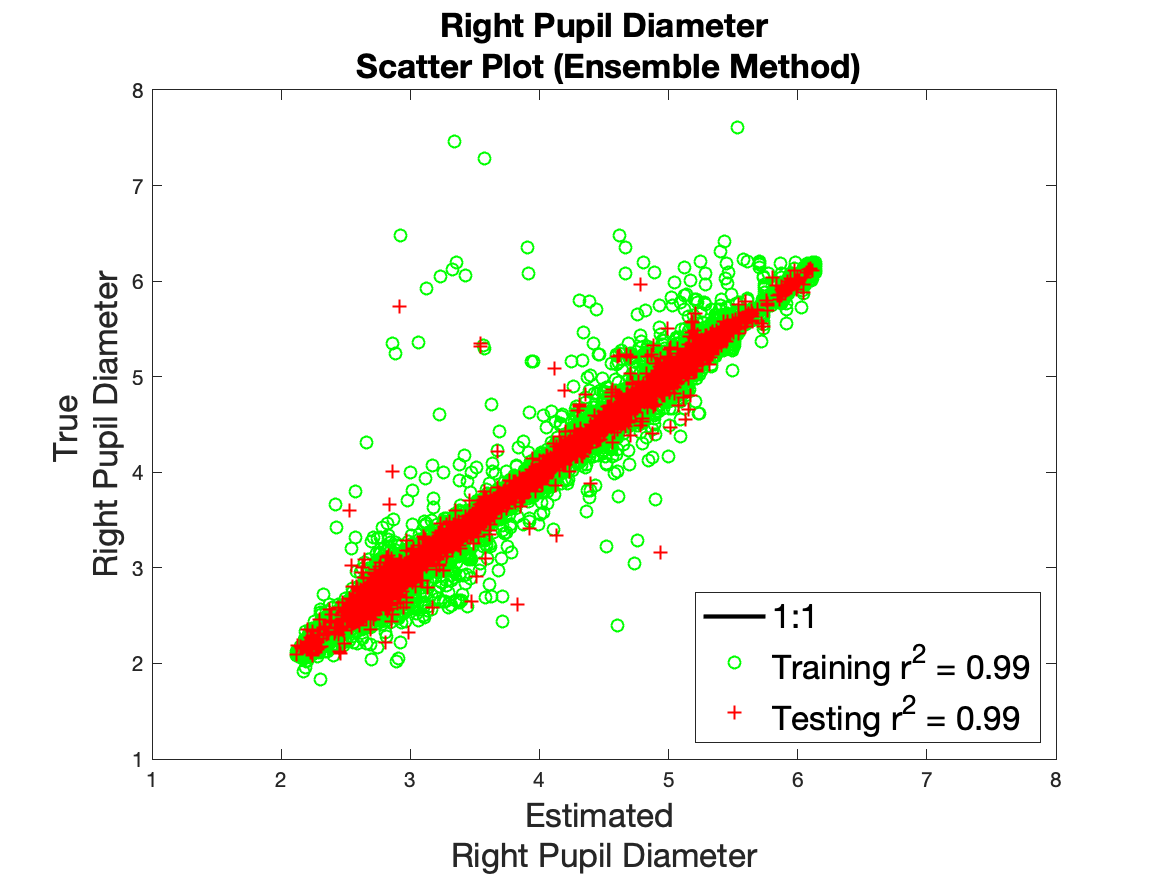
\includegraphics[width=0.48\textwidth]{./scatterPlots/RightPupilDiameter_Ensemble_Scatter2.png}\label{fig:OPMb}
  \caption{Plots for the pupil diameter prediction using model from opposite eye data. Pupil diameters are in millimeters(\textbf{a}) True vs estimated left pupil diameter using the right pupil diameter model. (\textbf{b}) True vs estimated right pupil diameter using the left pupil diameter model.
  }
  \label{fig:OPM}
\end{figure}

\subsection{The Illuminance Model}

Figure \ref{fig:ILM} shows the results of the illuminance model. We just saw above that if we know the light intensity we can accurately predict the pupil diameter, so now we \lq invert' the experiment and ask the question, if we know the pupil diameter can we accurately estimate the light intensity?

The model used the pupil diameters, gyroscope, and accelerometer data as the predictors. The estimates were some-what accurate with correlation coefficients of 0.91 and 0.71 for the training and testing datasets, respectively. The top 2 predictors are the left and right pupil diameters, which agrees with first order considerations of the relationship between pupil diameters and external light levels. The next most important predictor was the acceleration in the z-direction (forward direction). Which may again be correlated with participant focus on obstacle navigation. 

\begin{figure}[!t]
  \centering
  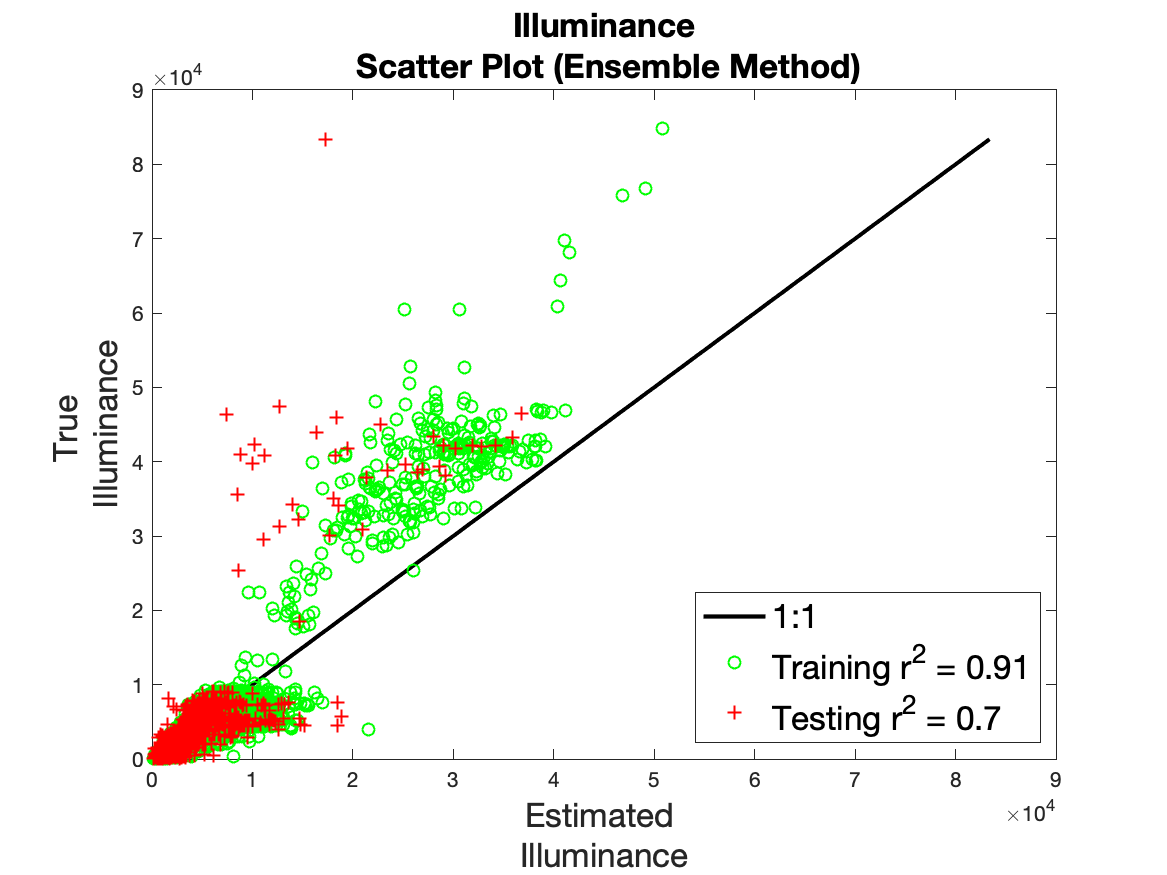
\includegraphics[width=0.48\textwidth]{./scatterPlots/Illuminance_Ensemble_Scatter2.png}\label{fig:ILMa}
  \hfill
  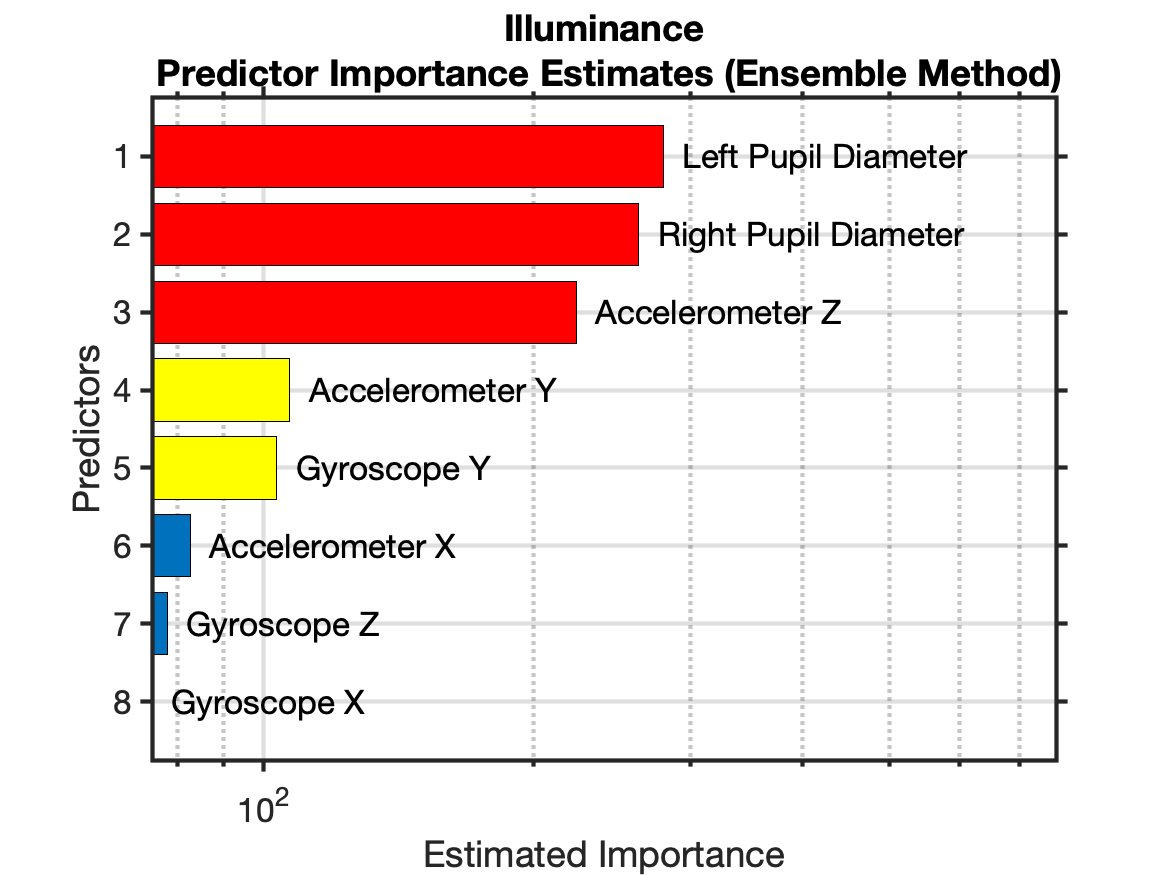
\includegraphics[width=0.48\textwidth]{./importanceRankings/IlluminanceEnsembleImpRankTall.png}\label{fig:ILMb}
  \caption{Plots for the illuminance model. (\textbf{a}) True vs estimated illuminance in lux. (\textbf{b}) Predictor importance estimates for the illuminance model.
  }
  \label{fig:ILM}
\end{figure}

\subsection{Pupil Diameter and Illuminance}

\begin{figure}[!b]
  \centering
  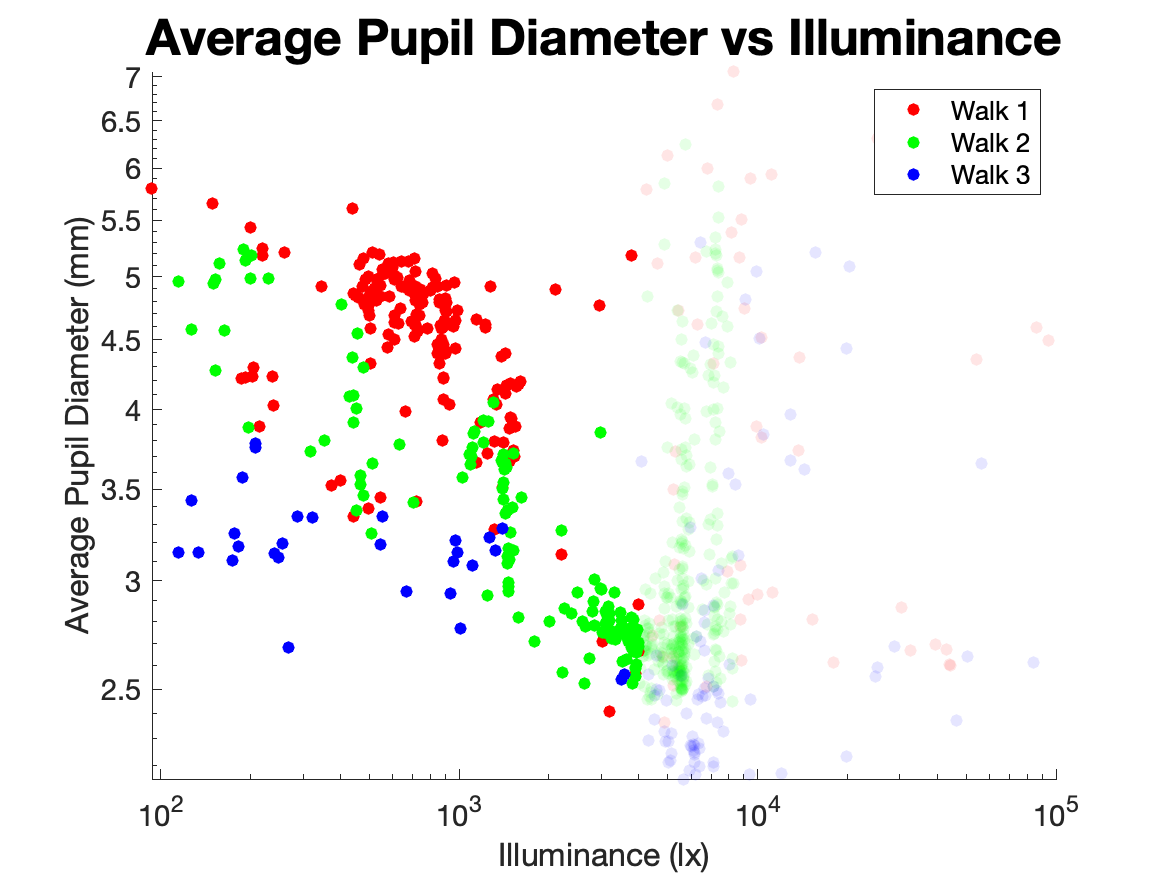
\includegraphics[width=0.32\textwidth]{./PDvsILM/APDvsILM.png}\label{fig:PDvsILMa}
  \hfill
  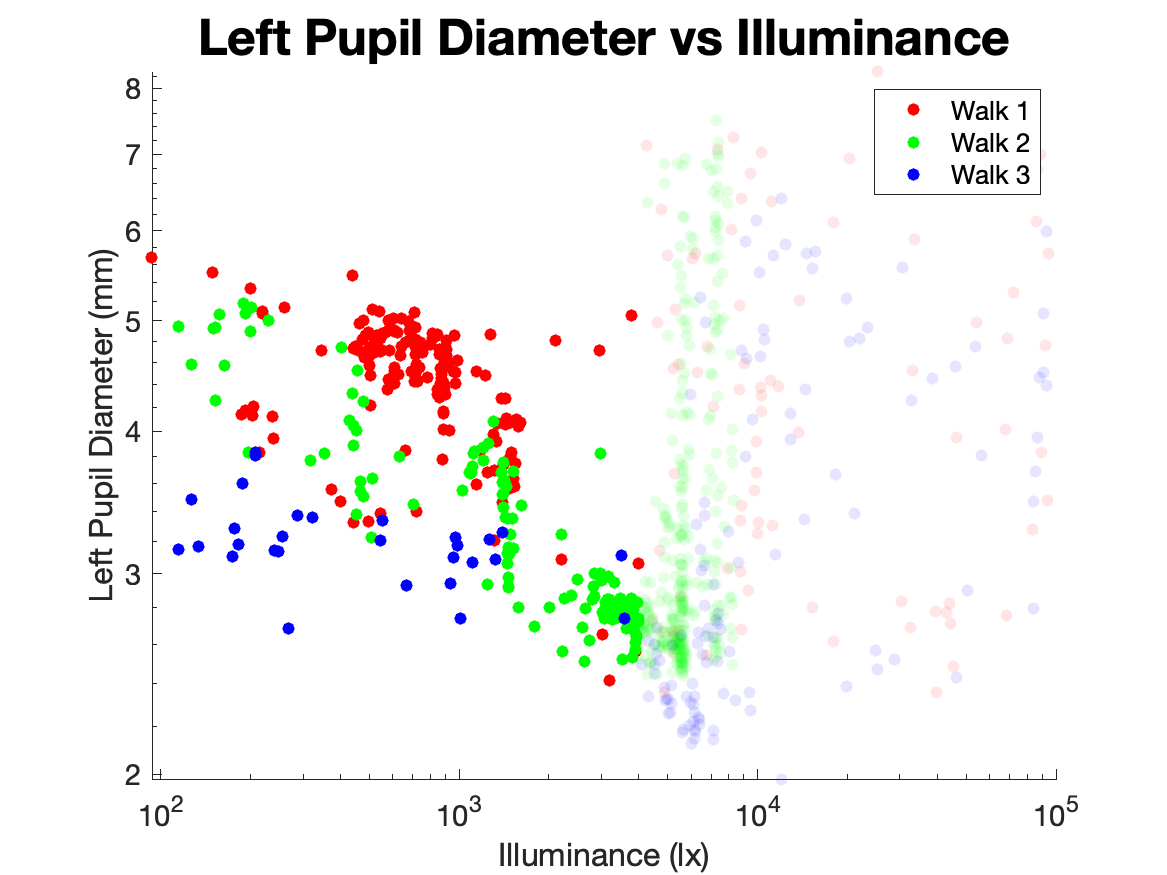
\includegraphics[width=0.32\textwidth]{./PDvsILM/LPDvsILM.png}\label{fig:PDvsILMb}
  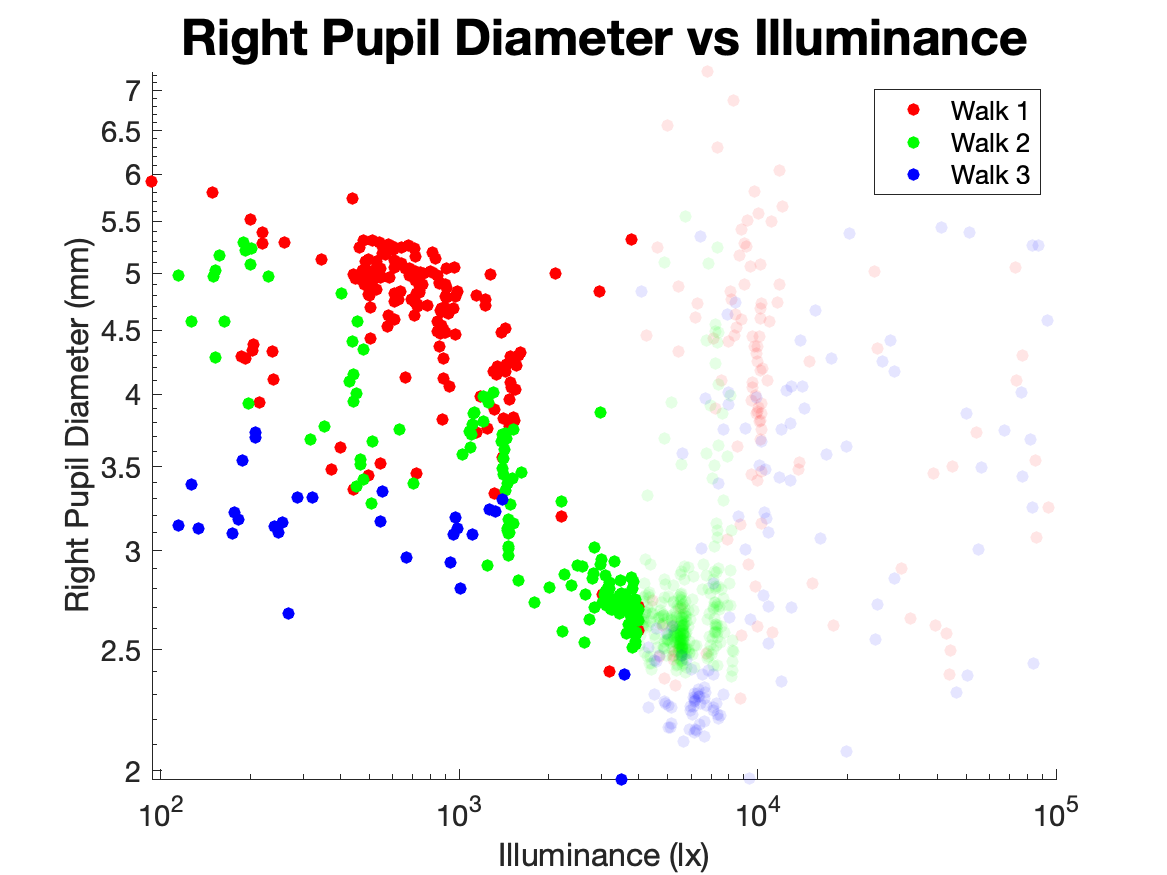
\includegraphics[width=0.32\textwidth]{./PDvsILM/RPDvsILM.png}\label{fig:PDvsILMc}
  \hfill
  \caption{Log scale scatter plots of the pupil diameters vs illuminance. Data from walks 1, 2, and 3 are distinguished by the colors red, green, and blue, respectively. Data points with low opacity have illuminance values above 4000 lx. Note below the 4000 lx mark the variables tend to have an inverse relationship. (\textbf{a}) Average pupil diameter vs illuminance. (\textbf{b}) Left pupil diameter vs illuminance. (\textbf{c}) Right pupil diameter vs illuminance.
  }
  \label{fig:PDvsILM}
\end{figure}

 \begin{figure}[!p]
    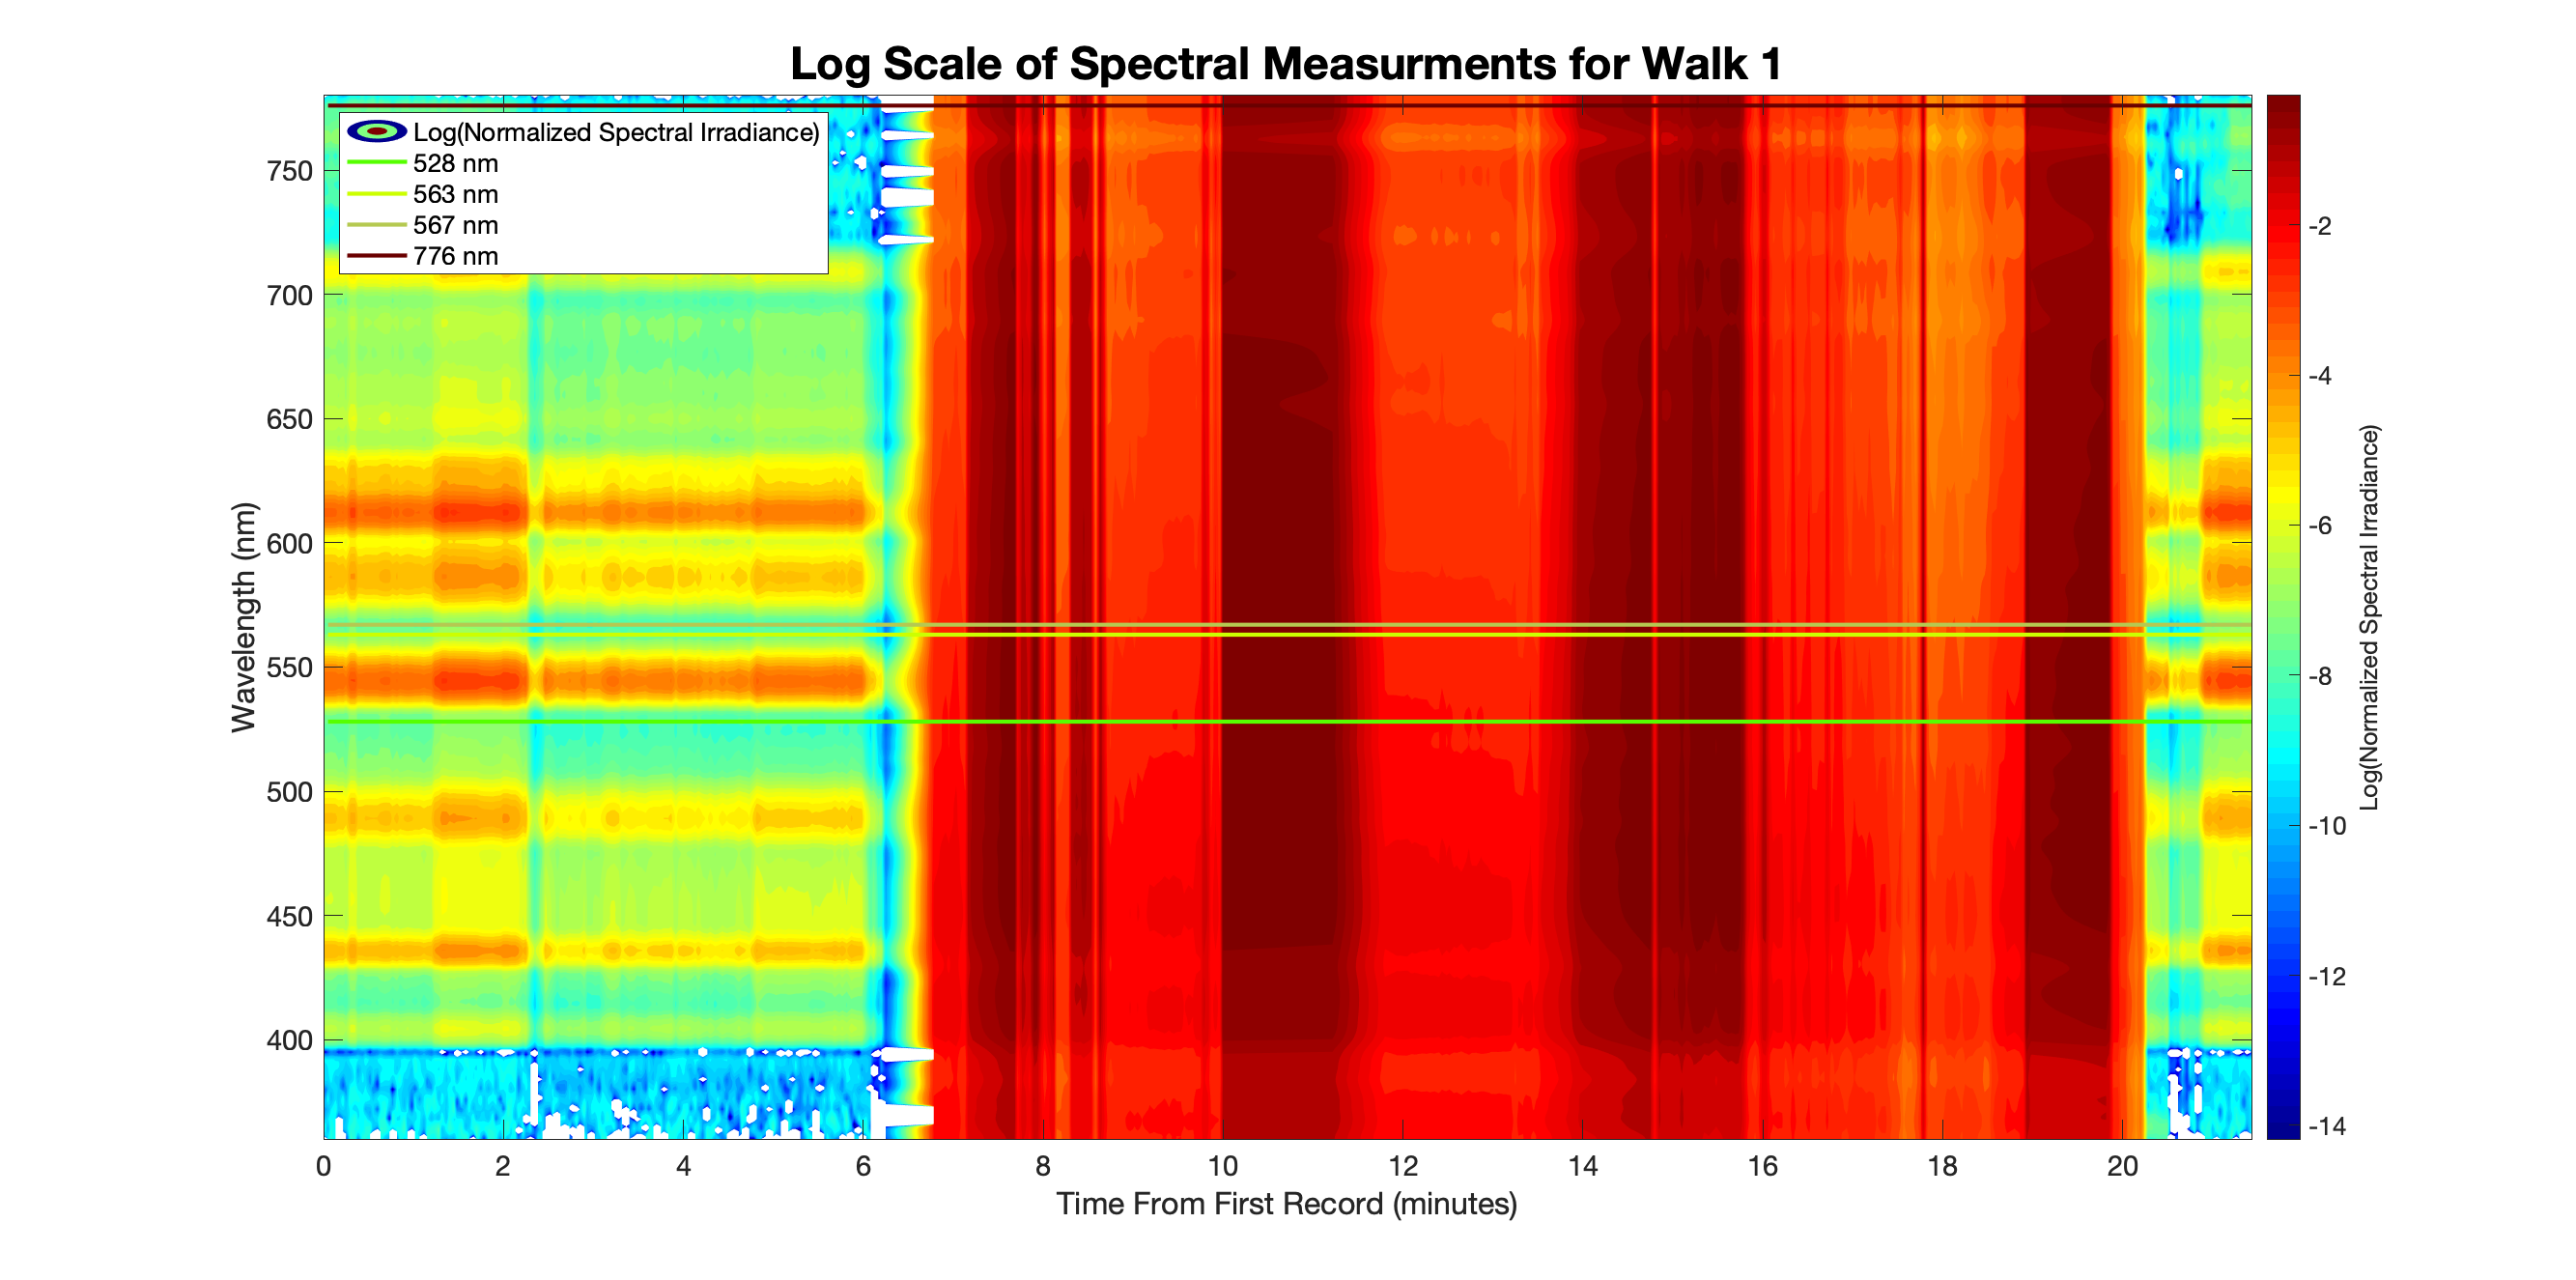
\includegraphics[width=\textwidth,keepaspectratio]{./spectrum/spectrum3_2logRun1.png}
    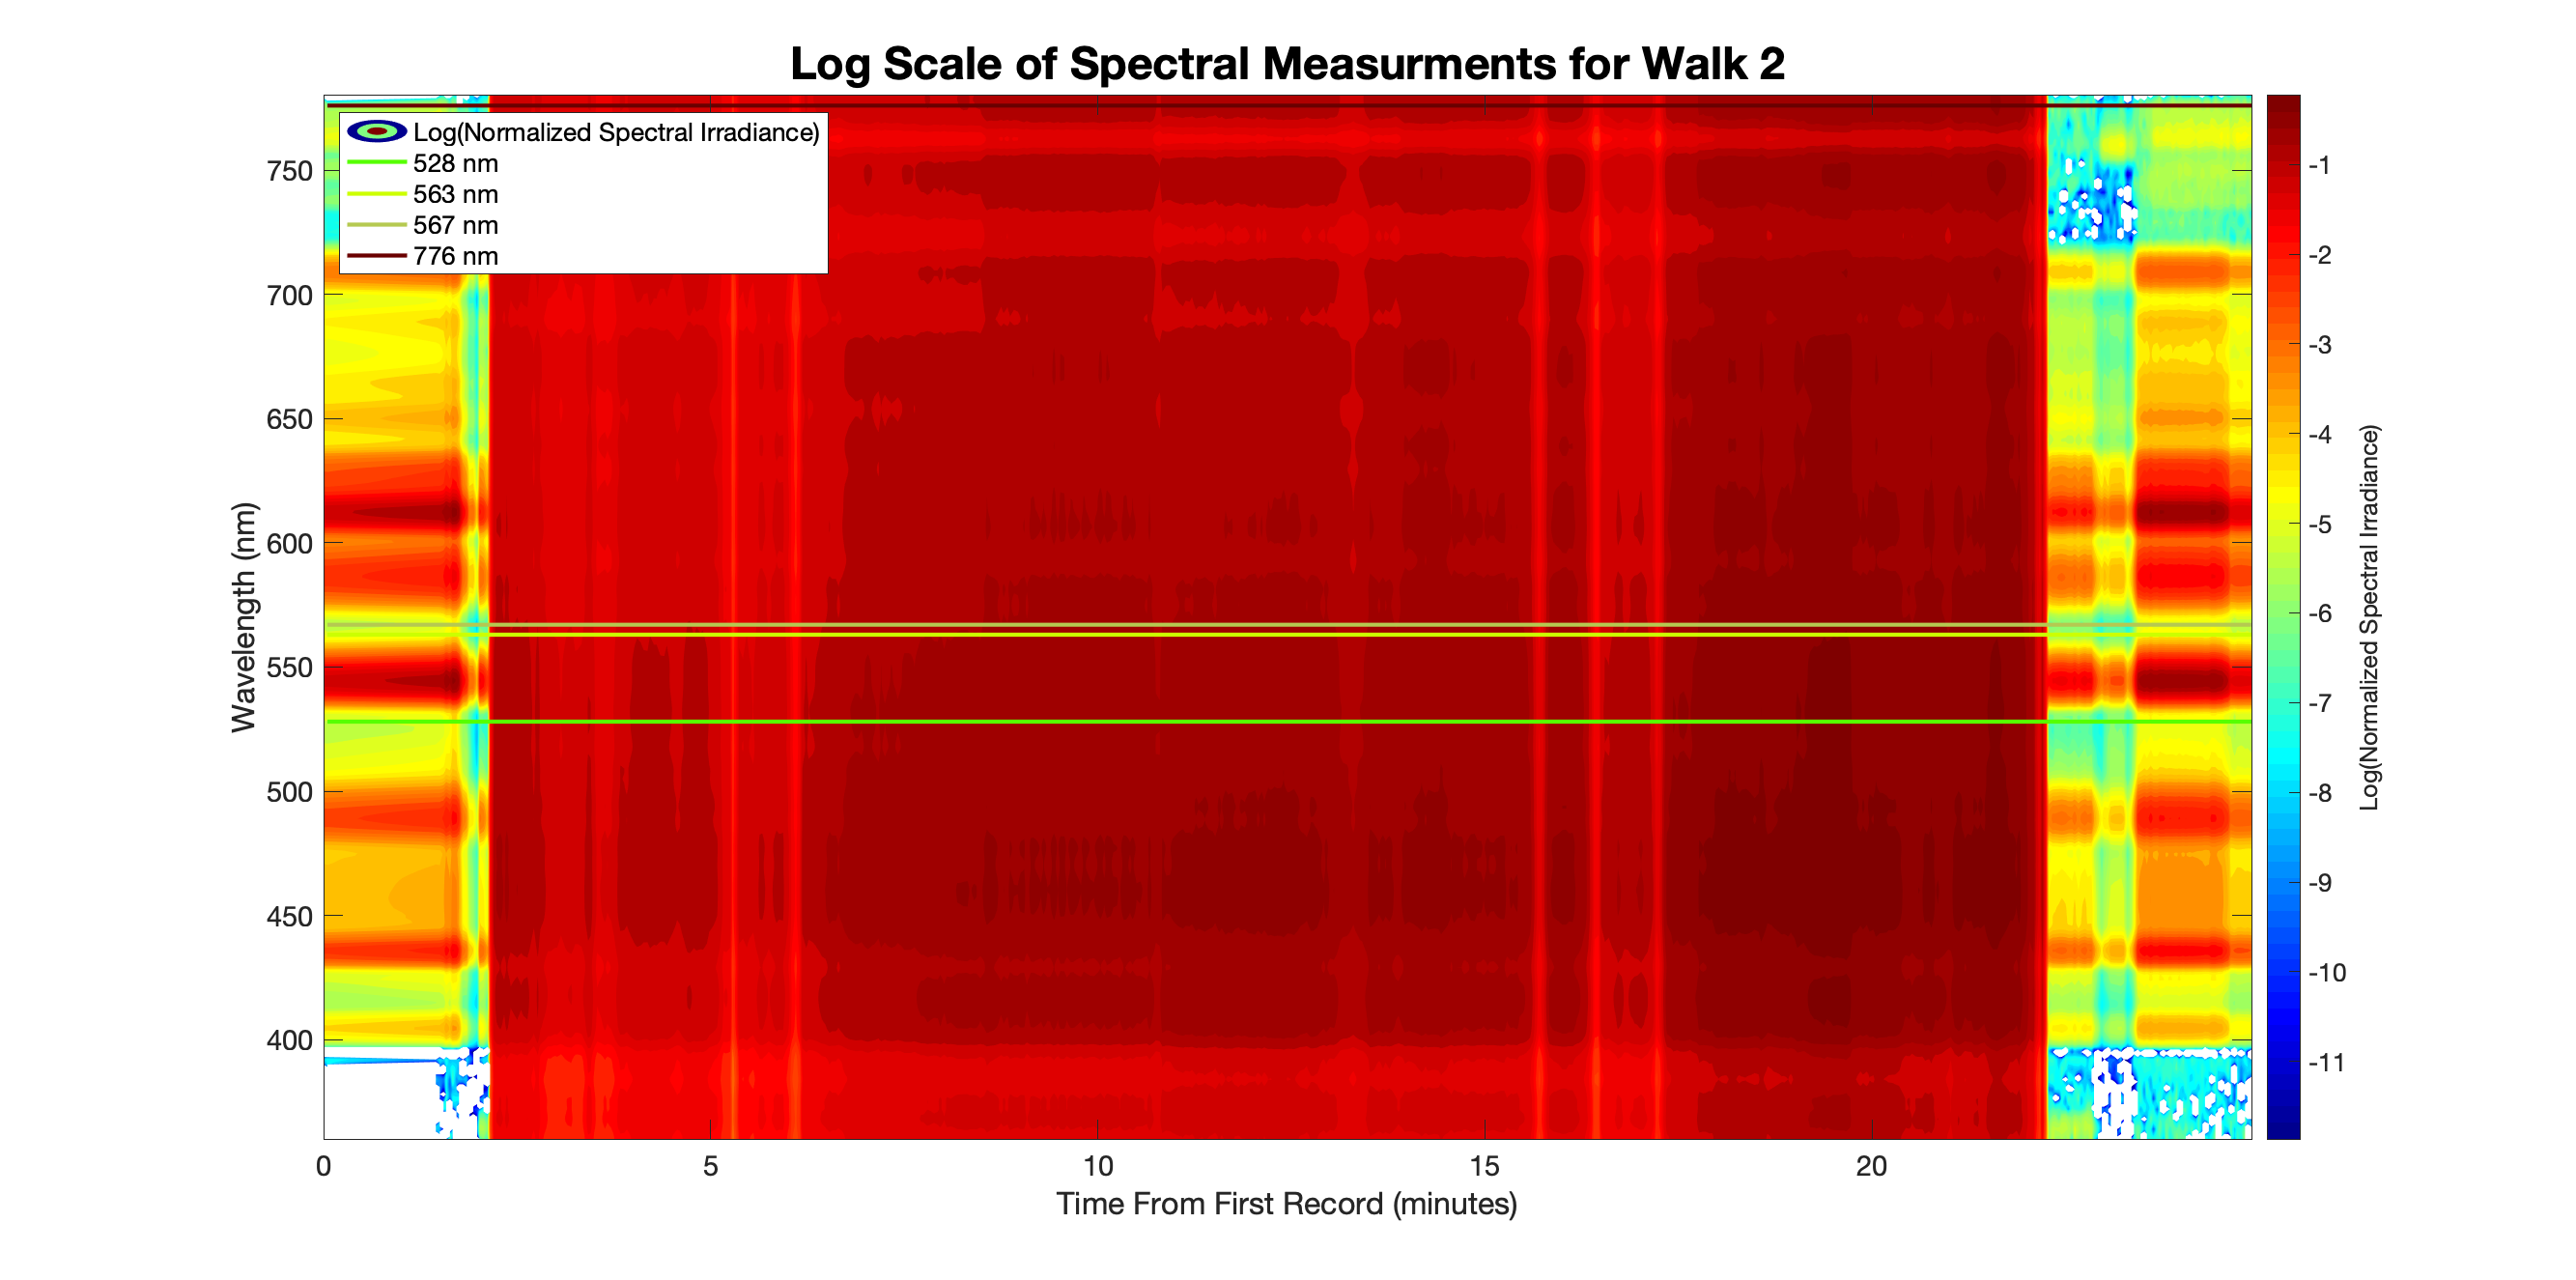
\includegraphics[width=\textwidth,keepaspectratio]{./spectrum/spectrum3_2logRun2.png}
    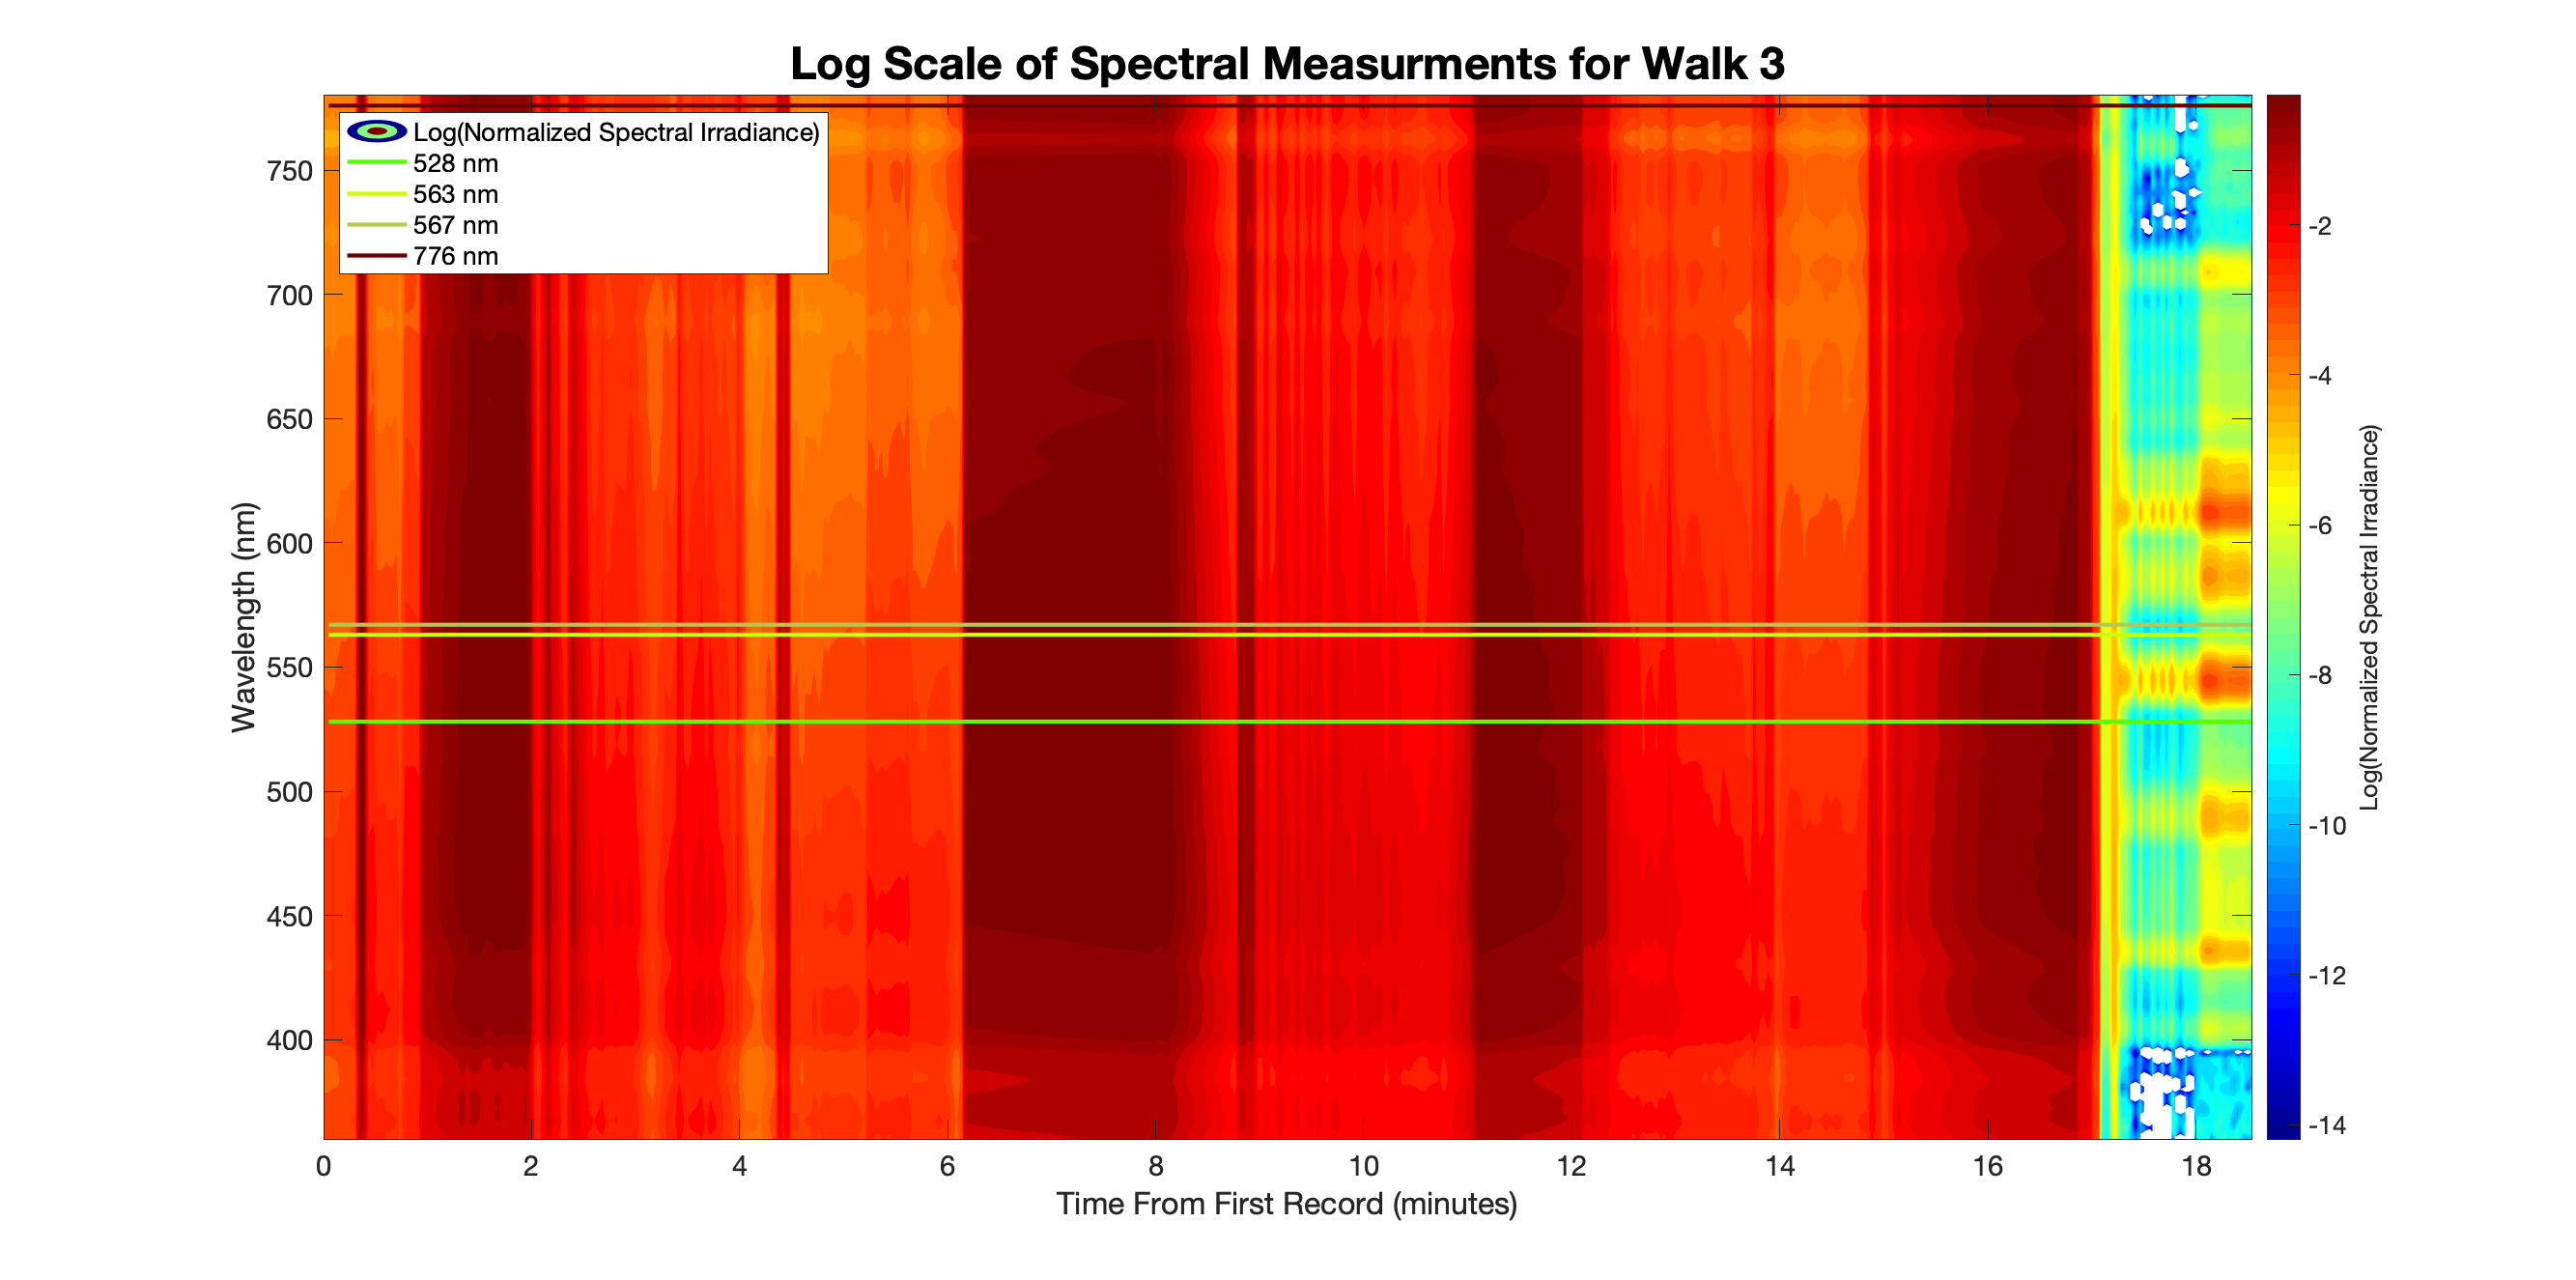
\includegraphics[width=\textwidth,keepaspectratio]{./spectrum/spectrum3_2logRun3.png}
    
    \caption{The log of the normalized spectral irradiance at every time step for all walks is plotted. The irradiance is normalized prior to taking log by dividing all values by the maximum spectral irradiance within each walk. Relative sizes of irradiance values are indicated by the colorbar. Spectral lines at 528, 563, 567, and 776 nm represent wavelengths of the most important predictors for the pupil diameter models.(\textbf{a}) Walk 1 measurements during late afternoon ($\approx$ 4PM). (\textbf{b}) Walk 2 measurements during morning ($\approx$ 8:30 AM). (\textbf{c}) Walk 3 measurements during late afternoon ($\approx$ 4PM).}
    
    \label{fig:specLog}
\end{figure}

In a first order consideration, we can expect the pupil diameter to be inversely proportional to the illuminance. This is depicted in Figure \ref{fig:PDvsILM}, which gives 3 scatter plots of the average, left, and right, pupil diameters vs illuminance. At low illuminance values, the expected inverse relationship is apparent. At higher values ($\gtrsim$ 4000 lux) this expectation fails. The lack of a clear relationship between the two variables in all situations is likely the main contributor to the failure of previous models (Figure \ref{fig:oldModels}). 

\subsection{The Environment}

The normalized spectral irradiance at every time step for each trial is given in Figure \ref{fig:specPD}. Normalized values were computed by dividing all irradiance values by the largest irradiance within each trial. Spectral lines are plotted for 528, 563, 567, and 776 nm, based on the top 3 most important predictors across all pupil diameter models (see Figures \ref{fig:APD}b, \ref{fig:LPD}b, \ref{fig:RPD}b, \& \ref{fig:PDD}b). Where predictors of the spectral irradiance at 561, 562, and 568 nm were disregarded in lieu of the irradiance at 563 and 567 nm. 

Temporal discontinuities in the spectra are due to those time intervals in which the participant walked in and out of shaded areas and/or away from the sun, which resulted in orders of magnitude differences in the spectral irradiance. Figure \ref{fig:specLog} depicts the normalized spectral irradiance plotted on a log scale. Time intervals colored predominately red represent outdoor spectra, while more colorful intervals are indoor.

\section{Limitations}

The high level of infrared noise caused significant drawbacks in the data analysis. Further developments may require light intensities and spectra to be within a non-disruptive range. Another solution may be to utilize an eye tracking instrument which uses visible light to estimate the pupil diameters.

\section{Future Directions}

Pupil size along with other autonomic responses such as heart rate variability, galvanic skin response, and core temperature changes have been associated with cognitive load and performance \cite{PupilLoad1,PupilLoad2,PupilLoad3,PupilLoad4,HRVreview, GSR, tempLoad}. Although cognitive load is a significant contributor to the provocation of these responses, in a dynamic outdoor environment and while performing a physical activity (such as walking or cycling) it is not always clear which responses were due to external stimuli or cognitive status. Using a similar approach to the one used here, future data collection will expand the number of participants, environments, cognitive tasks, and biometric sensors. 

Looking forward, multiple participants will allow for the assessment of the inter-person variability of the models, including parameters such as age and body composition. Different environments will vary in light intensity, air quality, elevation, and temperature. Environmental variables can be measured using mobile weather stations mounted on a participant or bicycle. Other environmental sensors such as a video camera, microphone, and LIDAR can indicate dynamic field situations and track events. Tasks such as walking and cycling will be performed. Cyclist performance can be assessed via bicycle speed and biometric data. Biometrics such as electroencephalography (EEG), heart rate (ECG), galvanic skin response (GSR), body temperature, electromyography (EMG), blood oxygen level, and respiration will be considered and modeled. The ranking of predictor importance for these biometric models can help identify important relationships between environmental stimuli and different autonomic responses.

\section{Conclusions}

Past formulae for predicting pupil diameter mainly considered total ambient light levels via luminance \cite{PupilModels, StanleyPupilMvModel, HolladayPupil1vModel, CrawfordPupil1vModel, MoonPupil1vModel, deGrootPupil1vModel, BlackiePupil1vModel, BartenPupilMvModel}, these models could not capture the fully multi-variate and non-linear dependence of pupil diameter on the environmental state, and consequently had poor generalization. When considering the spectrum of light from 360 -- 780 nm (ultra-violet to near infrared) in lieu of the luminance, we were able to derive a very accurate empirical machine learning model which can predict pupil diameters with a minimum fidelity of 96.9\%. The machine learning also allowed us to identify that the most important wavelengths in predicting the pupil diameters were around 562 nm (green), which is near the peak absorbance of the long-wave photo-receptive cones (\hbox{562.8 $\pm$ 4.7 nm}) \cite{BowmakerCones}.

\section{Supplementary Materials}

Codes and raw data used in this experiment are available at the LightOcular GitHub repository: \url{https://github.com/mi3nts/LightOcular}

All data used in this experiment is publicly available at the following Zenodo data store: \url{https://zenodo.org/record/3354602#.XUi9wJNKjVp}. doi: 10.5281/zenodo.3354602

\vspace{6pt} 

%\authorcontributions{conceptualization, David J. Lary; methodology, Shawhin Talebi, David J. Lary, and Lakitha O. H. Wijerante; software, Shawhin Talebi, David J. Lary, and Lakitha O. H. Wijerante; validation, Shawhin Talebi and David J. Lary; formal analysis, Shawhin Talebi and David J. Lary; investigation, Shawhin Talebi and David J. Lary; resources, David J. Lary; data curation, Shawhin Talebi; writing—original draft preparation, Shawhin Talebi and David J. Lary; writing—review and editing, Shawhin Talebi and David J. Lary; visualization, Shawhin Talebi and David J. Lary; supervision, David J. Lary and Lakitha O. H. Wijerante; project administration, David J. Lary; funding acquisition, David J. Lary”}

%\funding{This research was funded by USAMRMC Award Number W81XWH-18-1-0400.}

%\conflictsofinterest{The authors declare no conflict of interest.} 

\bibliography{LightOcular}
\bibliographystyle{unsrtnat}

\end{document}

